\documentclass[twocolumn,aps,prd,reprint]{revtex4-1}
\usepackage{blindtext}
%\usepackage[justification=centering]{caption}
\usepackage{graphics,setspace,enumitem,graphicx,textpos,placeins,float}
\begin{document}
\graphicspath{{AnnWang/}}
\bibliographystyle{plain}
\title{	CMS Trigger Studies for Supersymmetry Searches with the Razor Variables}
\author{Ann Wang}
\email{amwang@caltech.edu}
\author{Javier Duarte}
\author{Maria Spiropulu}
\affiliation{California Institute of Technology}
%\begin{spacing}{1.2}

\begin{abstract}
Supersymmetric extensions of the Standard Model are the next steps towards discovering new physics and explaining phenomena such as dark matter. At the Compact Muon Solenoid (CMS) Detector, high energy events from the Large Hadron Collider (LHC) can be studied for signs of supersymmetry (SUSY). One technique for SUSY searches employs razor kinematic variables, which help separate SUSY events from Standard Model background. Due to the high number of events produced at the LHC, however, two trigger levels, Level 1 and the High Level Trigger (HLT), must be implemented at the CMS detector to select for physically interesting events to record. Several selection criteria, which include both angular and energy information, are studied in the context of the razor variables at these trigger levels. A detailed analysis of jet clustering algorithms is also conducted for the HLT.
\end{abstract}
\maketitle
\section{Introduction}
Dark matter composes approximately 80\% of all matter in the universe, but the composition of dark matter is poorly understood. Currently, there is no viable candidate for a particle that makes up dark matter \cite{dark}. To address this problem, we can look to supersymmetry, which provides a particle candidate for dark matter, as well as a solution to the fine-tuning problem \cite{primer}. Supersymmetric extensions of the Standard Model (SUSY) may provide the key to understanding the physics of the universe. With the Compact Muon Solenoid (CMS) general-purpose detector, scientists at the Large Hadron Collider (LHC) are conducting supersymmetry searches. The CMS detector is composed of several subdetectors, including a lead-tungstate-crystal electromagnetic calorimeter, a hadronic calorimeter, a silicon tracker, and a muon system composed of drift tubes, cathode strip chambers, and resistive plate chambers \cite{lhc_detectors}. 
The 2015 run of the LHC will have technical improvements that will enable the machine to achieve proton-proton collisions at higher energies. The events reaching the detector are large in number and include both interesting and uninteresting events, so a trigger system is implemented in order to select for interesting events. This trigger system has two levels that allow for data reduction down to a rate on the order of 100 Hz. The two levels include the Level-1 (L1), which is hardware-based, and the High Level Trigger (HLT), which is software-based. At both of these levels, kinematic variables, such as transverse momentum, as well as other identifying data, are only partially reconstructed to reduce CPU requirements \cite{hlt}. The filters at both levels must be carefully examined and tested to ensure that the data reduction is to adequate levels and that the efficiency of collecting interesting events, which may be compromised due to detector resolution, remains high. 
\par In the 2012 analyses, $M_{R}$ and $R^2$-based trigger selections were implemented at the HLT level for razor analyses \cite{talk}. The razor variables $M_{R}$ and $R^2$ are employed because they are able to distinguish SUSY from a background of Standard Model events. For example, if we consider two squarks that each decay to a quark and a stable, weakly interacting Lightest Supersymmetric Particle (LSP), the missing energy carried away by the LSP makes it difficult to reconstruct and identify this SUSY decay. For an all-hadronic analysis, if we cluster the jets into two hemispheres, $M_{R}$ is defined as $M_R = \sqrt{(|p^{j1}|+|p^{j2}|)^2-(p_z^{j1}+p_z^{j2})^2}$, where $p_{ji}$ is the momentum of the ith hemisphere. $R$ is defined as $R = M^R_T/M_R$, where $$M^R_T = \sqrt{\frac{E^{miss}_T(p_T^{j1}+p_T^{j2})-\vec{E}^{miss}_T\cdot(\vec{p}_T^{\,j1}+\vec{p}_T^{\,j2})}{2}},$$ and $E_T^{miss}$ is the missing transverse energy of the event. The razor variables are formulated such that the peak of $M_R$ is related to characteristic SUSY mass scales, and $R^2$ contains information about the energy carried away by the invisible particles as well as the visible quark momenta \cite{squark}. As a result, the razor variables have been an ideal tool in SUSY searches. 
\par The L1 and HLT trigger seeds for the razor analyses need to be revised before the 2015 run. We are currently investigating several options for the L1 menu as well as the HLT menu as the CMS collaboration moves forward with updates for the new run. 
%\begin{figure*}
%\caption{\label{fig:T2qq} (a) Top/antistop pair production, which serves as the main background. (b) Squark and antisquark pair production decaying to quark/antiquark and two LSPs. (c) Gluino pair production decaying to four quarks and two LSPs. (d) Stop/antistop pair production decaying to top/antitop and two LSPs.}
%\centering
 %\includegraphics[width=0.9\textwidth]{feynman_2.pdf}
%\end{figure*}
%\begin{figure*}
%\caption{\label{fig:T2qq} (a) Gluino pair production decaying to four quarks and two LSPs. (b) Squark and antisquark pair production decaying to quark/antiquark and two LSPs.}
%\centering
%\includegraphics[width=0.9\textwidth]{feynman_new.pdf}
%\end{figure*}
\begin{table}[h]
\renewcommand{\tabcolsep}{0.2cm}
\begin{tabular}{l*{3}{c}l}
Signals &      Pair-produced & Decay\\
\hline
T2qq & $\tilde{q}$ $\tilde{q}*$ & $q$ $\tilde{\chi}^0_1$ $\bar{q}$ $\tilde{\chi}^0_1$ \\
T2tt & $\tilde{t}$ $\tilde{t}*$  & $t$ $\tilde{\chi}^0_1$ $\bar{t}$ $\tilde{\chi}^0_1$ $\rightarrow$ $b$ $W^+$ $\tilde{\chi}^0_1$ $\bar{b}$ $W^-$ $\tilde{\chi}^0_1$\\
T1qqqq  & $\tilde{g}$ $\tilde{g}*$  & $q$ $q$ $\tilde{\chi}^0_1$ $\bar{q}$ $\bar{q}$ $\tilde{\chi}^0_1$\\
\end{tabular}
\caption[Table caption text]{Table of the SUSY signal models discussed. }
\label{table:signals}
\end{table}
\begin{figure}[h]
 %\centering
 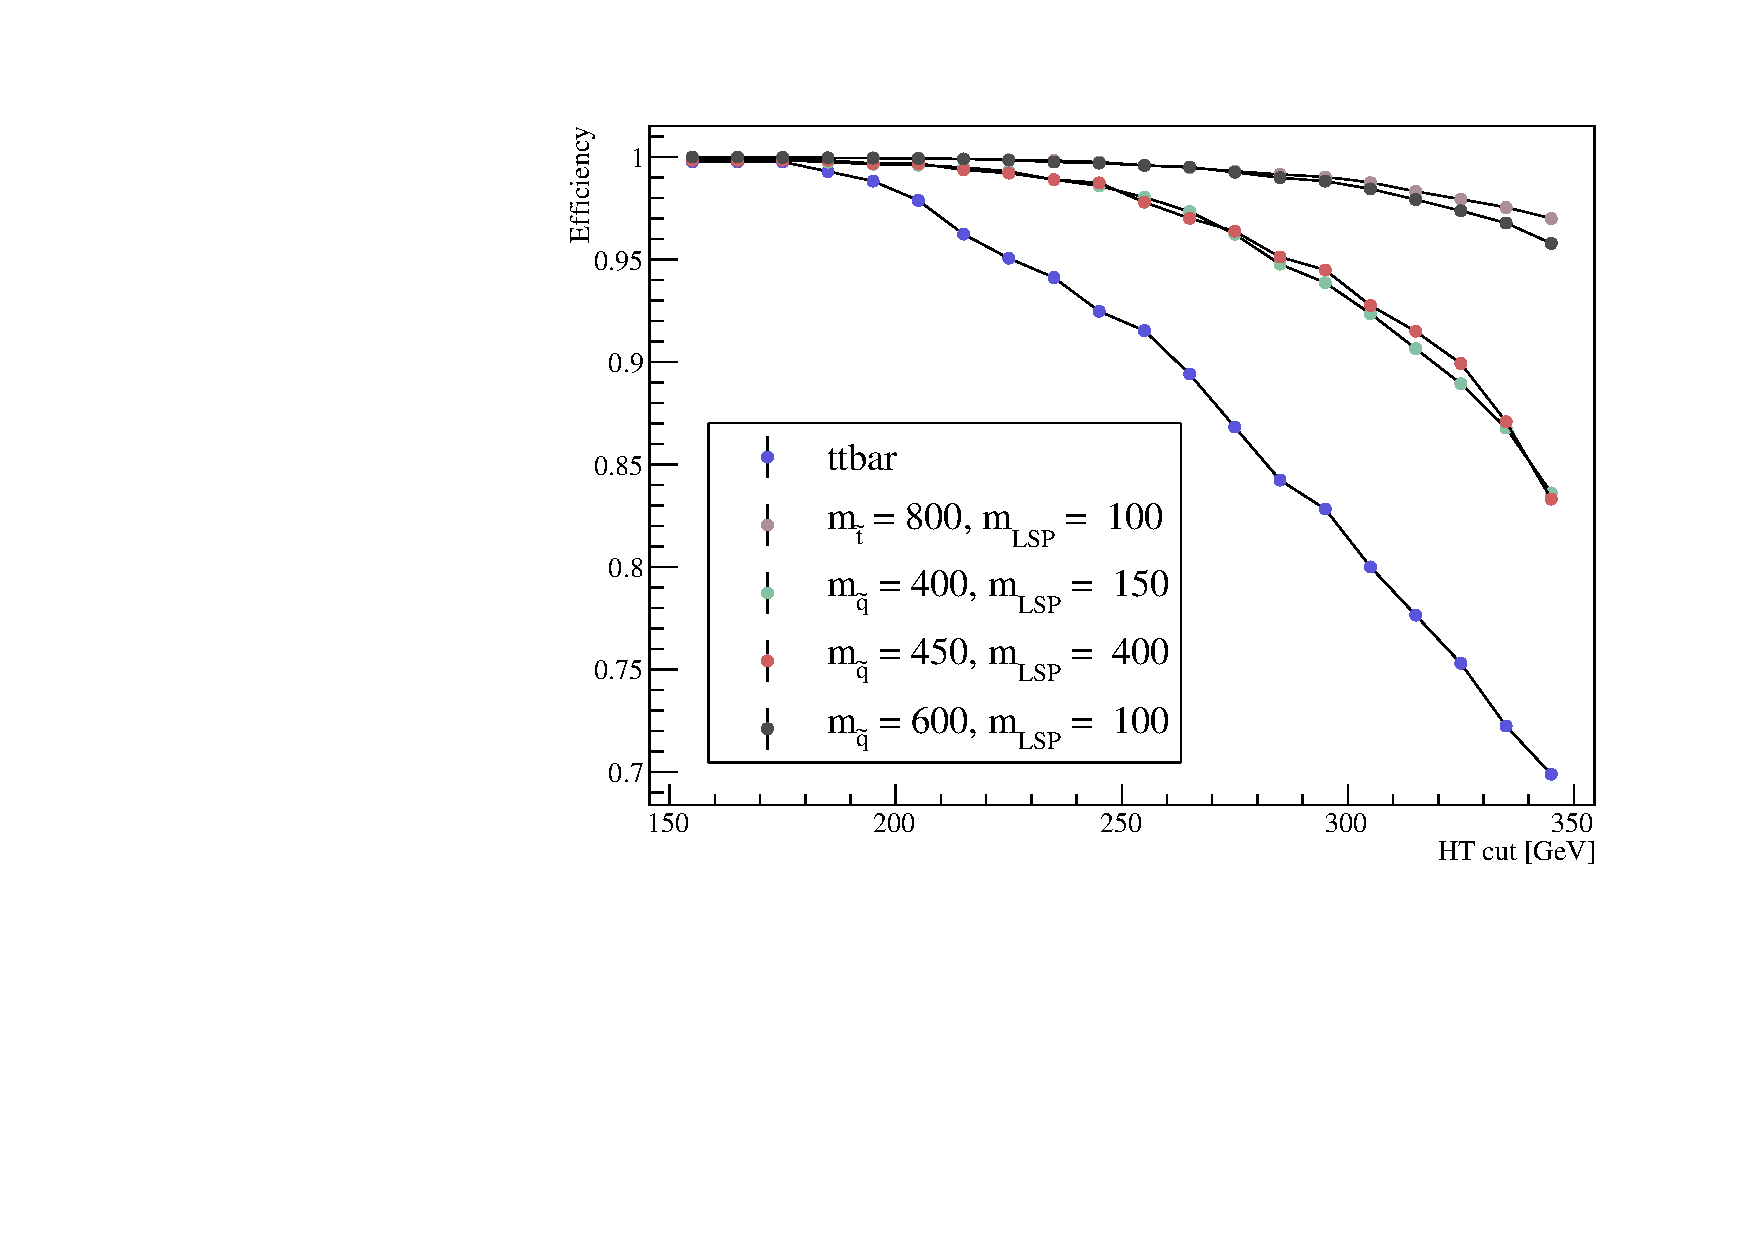
\includegraphics[width=0.5\textwidth]{efficiency.pdf}
\caption{\label{fig:eff_total} Total efficiency plotted for the five samples, over a region of 400 to 1450 in $M_R$ and 0.25 to 1.5 in $R^2$.}
\end{figure}
\begin{figure}
 %\centering
 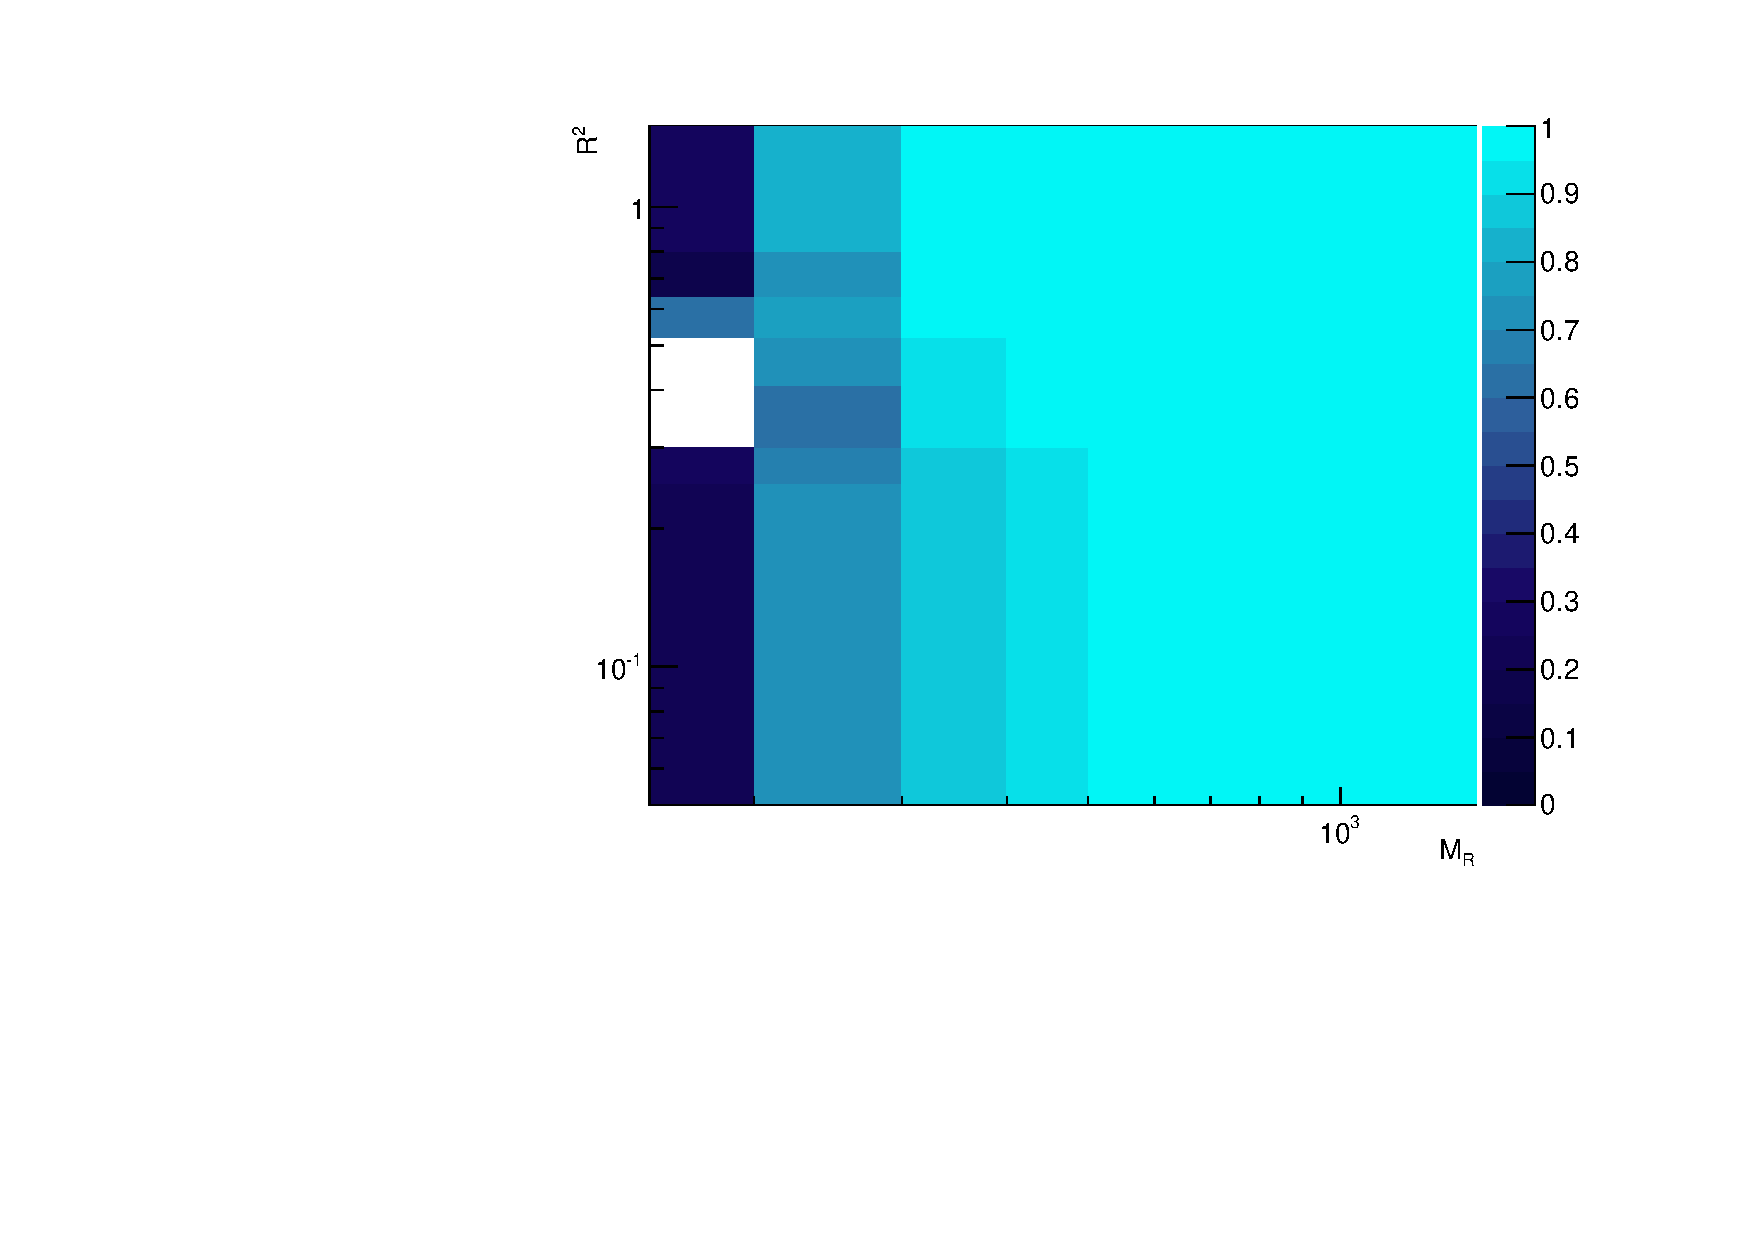
\includegraphics[width=0.45\textwidth]{ht200_file0.pdf}
\caption{\label{fig:eff_t2tt} 2D binned plot in efficiencies for $M_R$ and $R_2$ in T2tt, with $H_T>200$ GeV.}
\end{figure}
\begin{figure}
 %\centering
 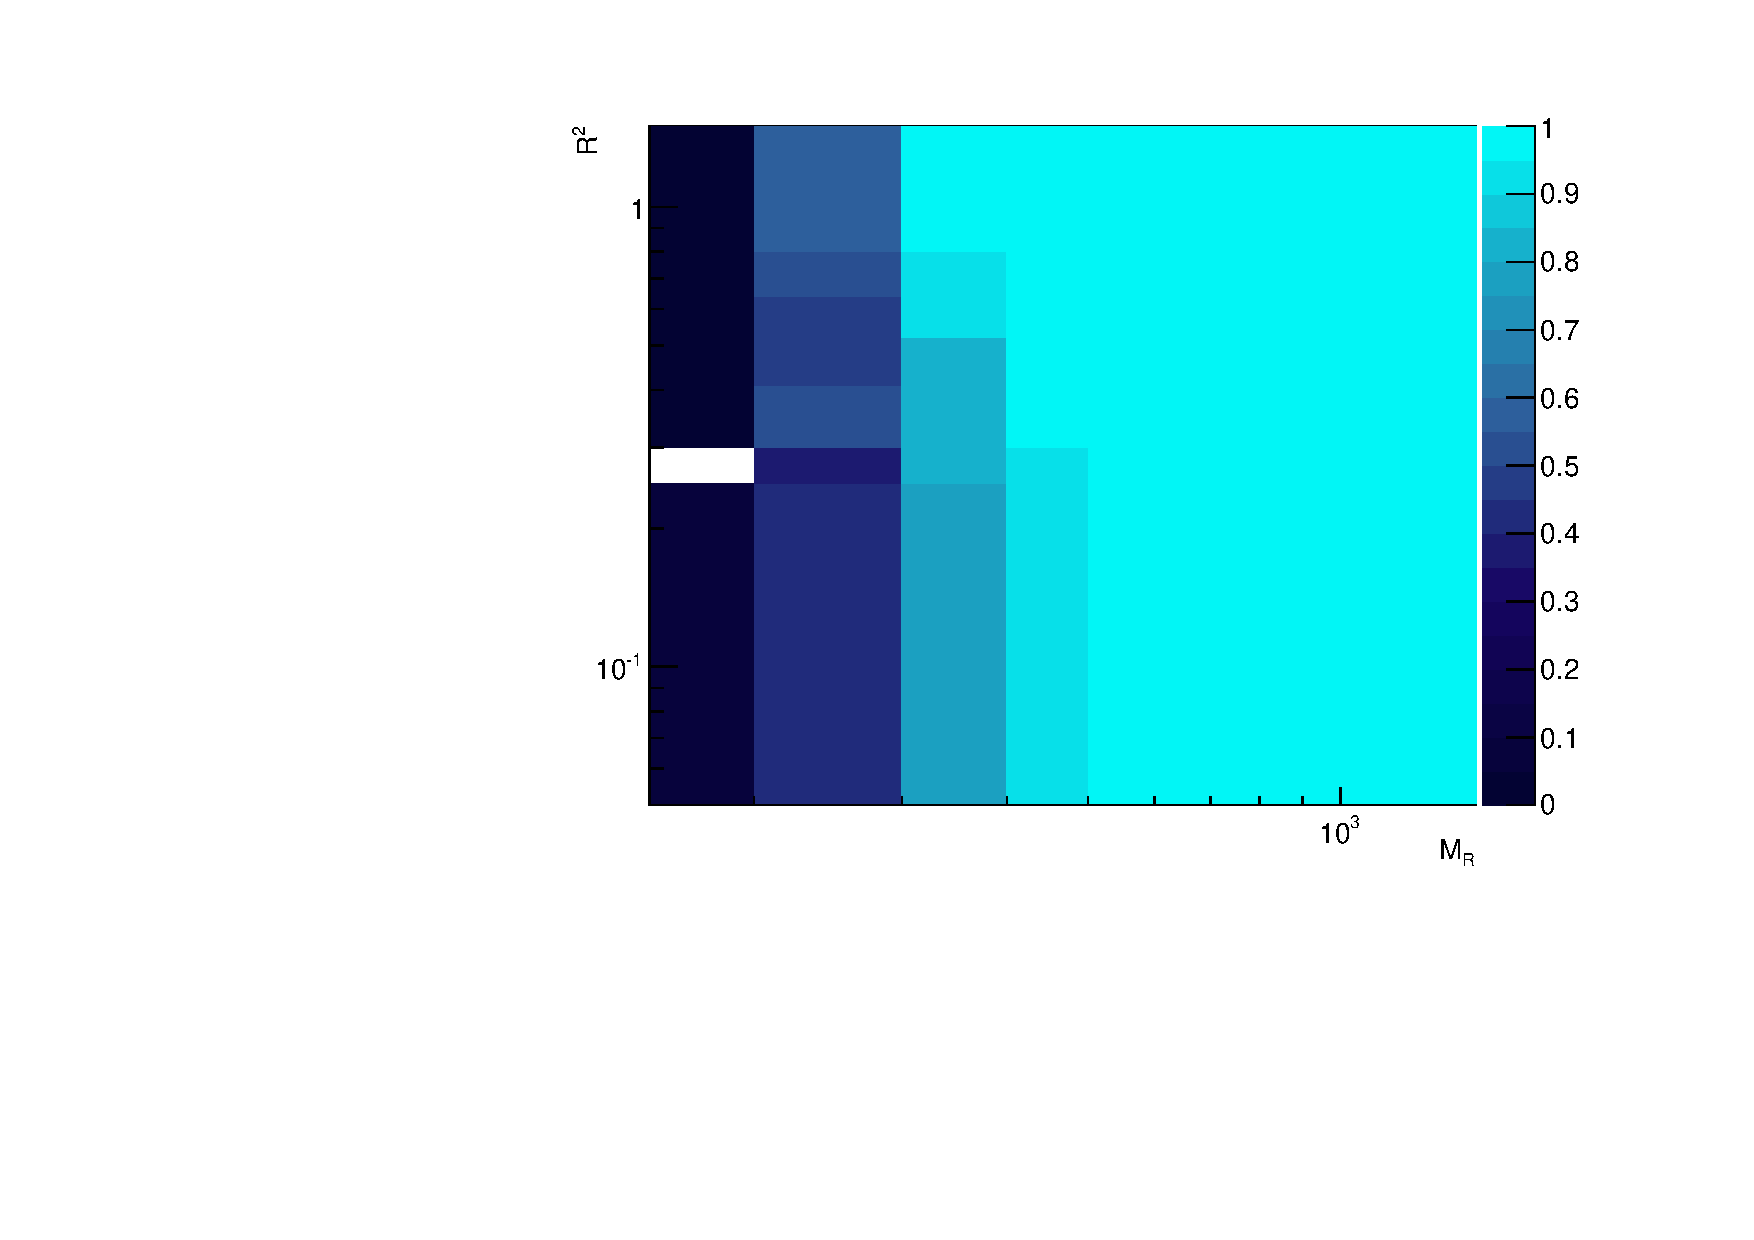
\includegraphics[width=0.45\textwidth]{ht200_file1.pdf}
\caption{\label{fig:eff_t211} 2D binned plot in efficiencies for $M_R$ and $R_2$ in T2qq with squark mass of 400 GeV and LSP mass of 150 GeV, with $H_T>200$ GeV. The z color axis refers to the efficiency.}
\end{figure}
\begin{figure}
 %\centering
 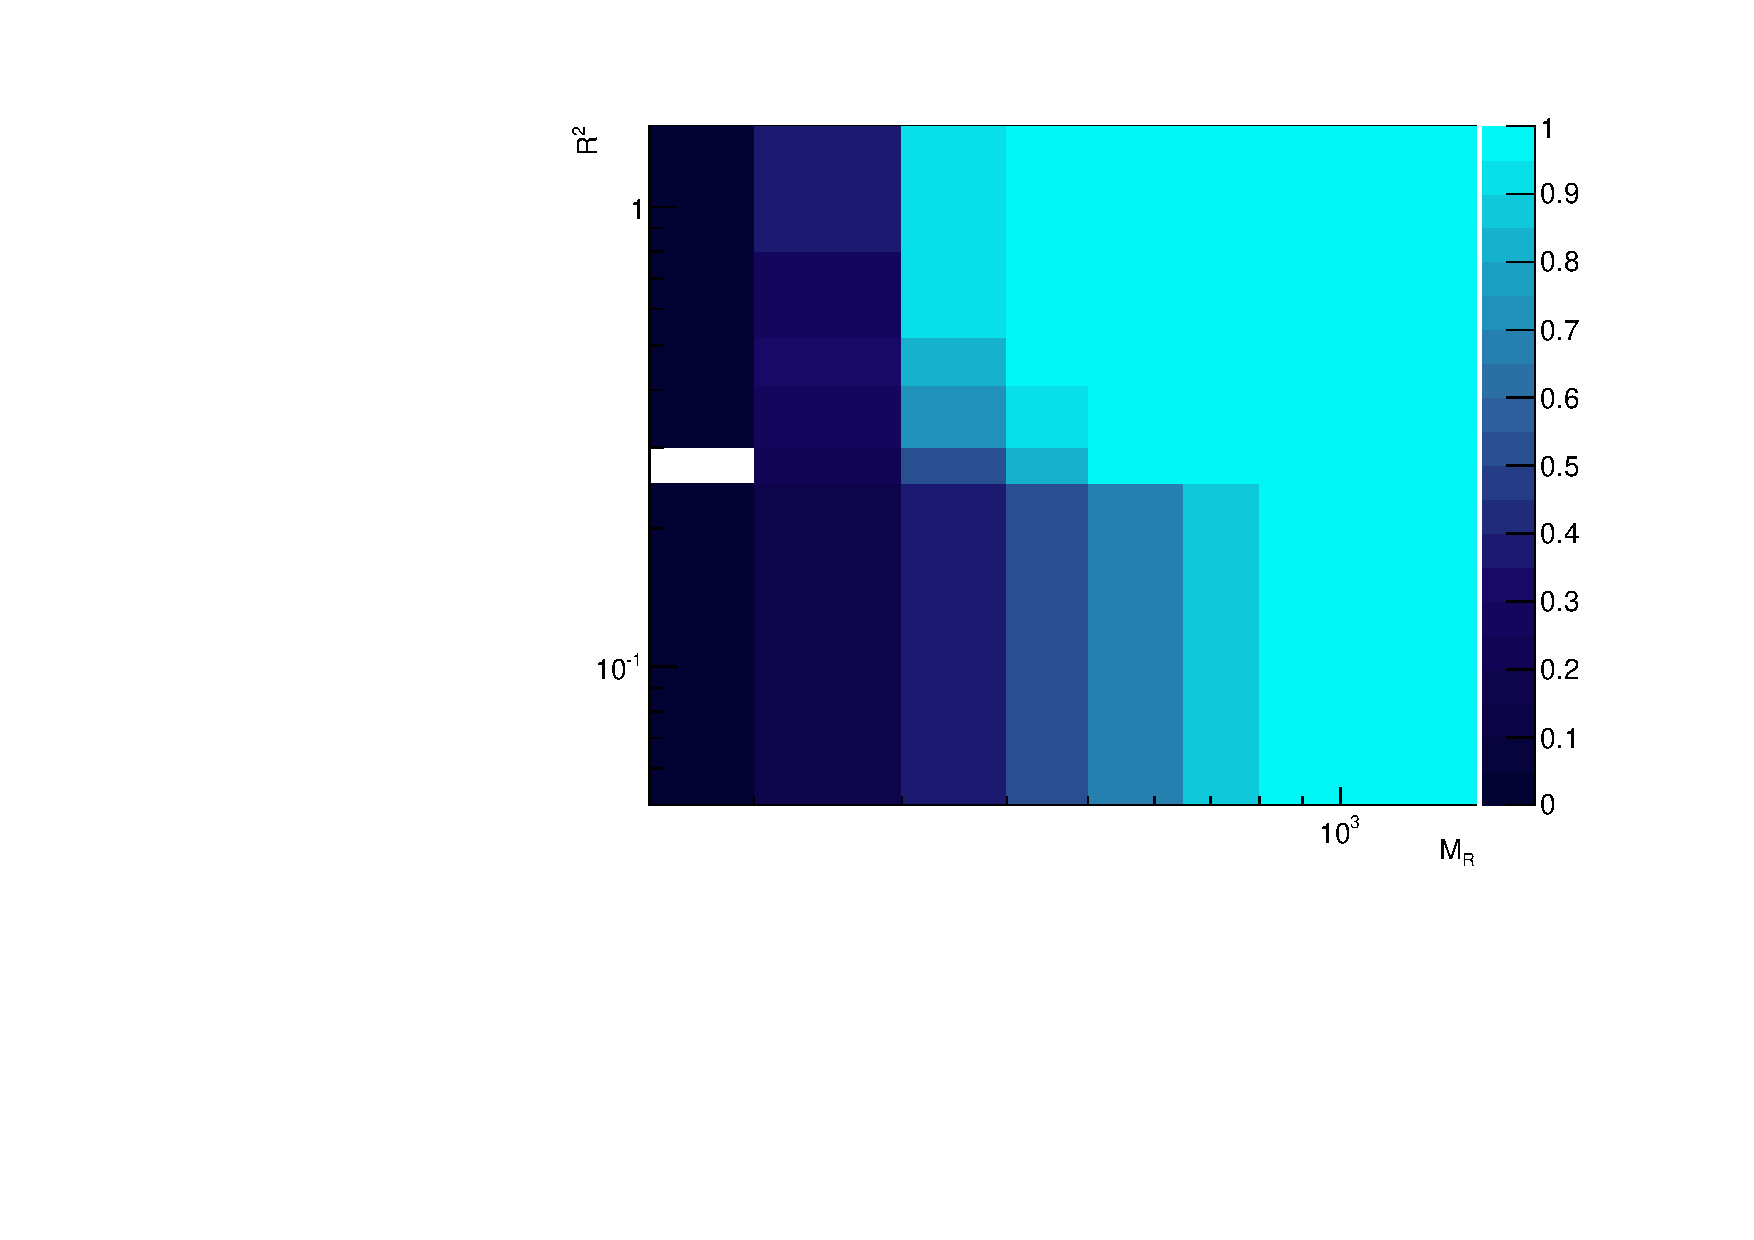
\includegraphics[width=0.45\textwidth]{ht200_file2.pdf}
\caption{\label{fig:eff_t2com} 2D binned plot in efficiencies for $M_R$ and $R_2$ in T2qq with squark mass of 450 GeV and LSP mass of 400 GeV, with $H_T>200$ GeV. The z color axis refers to the efficiency.}
\end{figure}
\begin{figure}[h]
 %\centering
 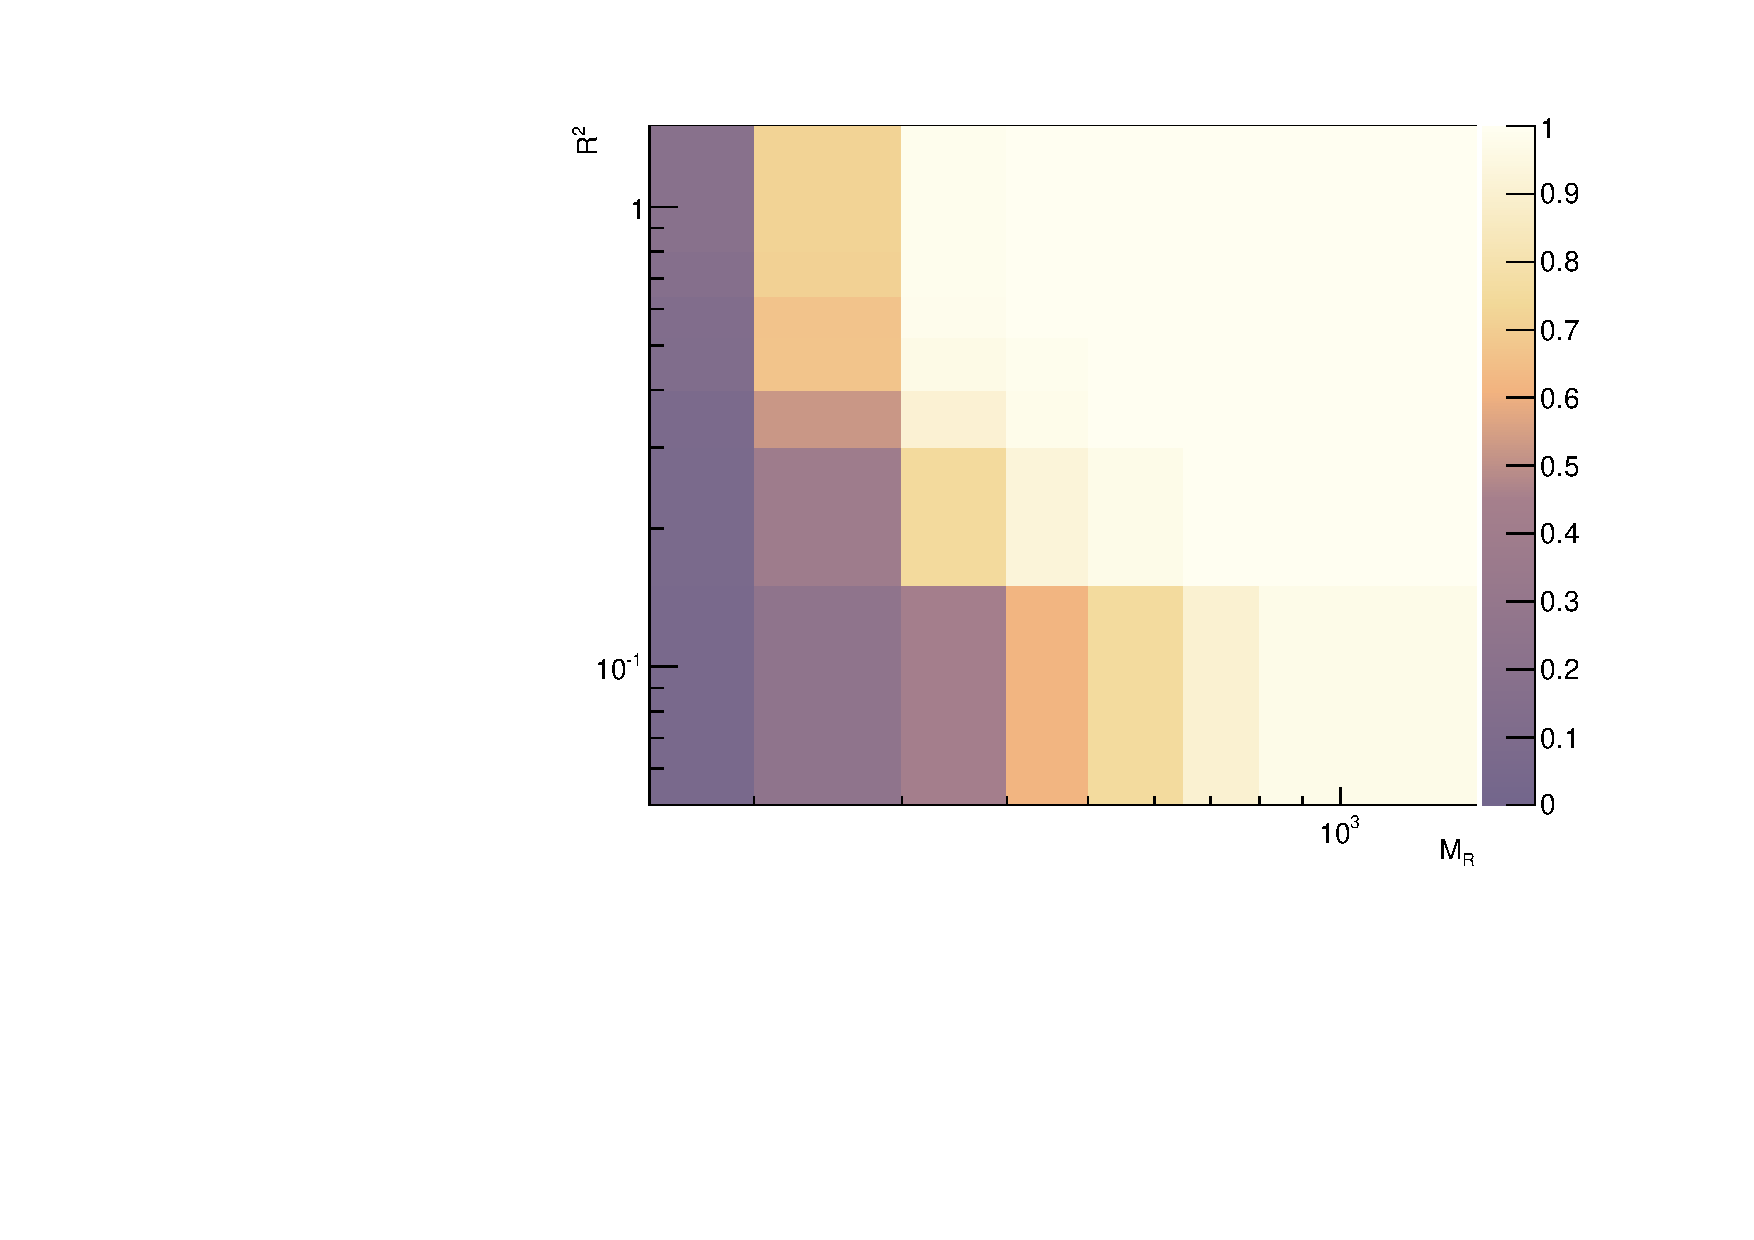
\includegraphics[width=0.45\textwidth]{newtrigger_OR_ht200_file2.pdf}
\caption{\label{fig:comp} 2D binned plot in efficiencies for $M_R$ and $R_2$ in T2qq with squark mass of 450 GeV and LSP mass of 400 GeV, with $H_T>200$ GeV OR  $H_T>125$ GeV \& single jet $p_T>120$ \& two jets with $p_T>30$ \& $\Delta\phi<$2.6 radians. The z color axis refers to the efficiency.}
\end{figure}
\begin{figure}[h]
 %\centering
 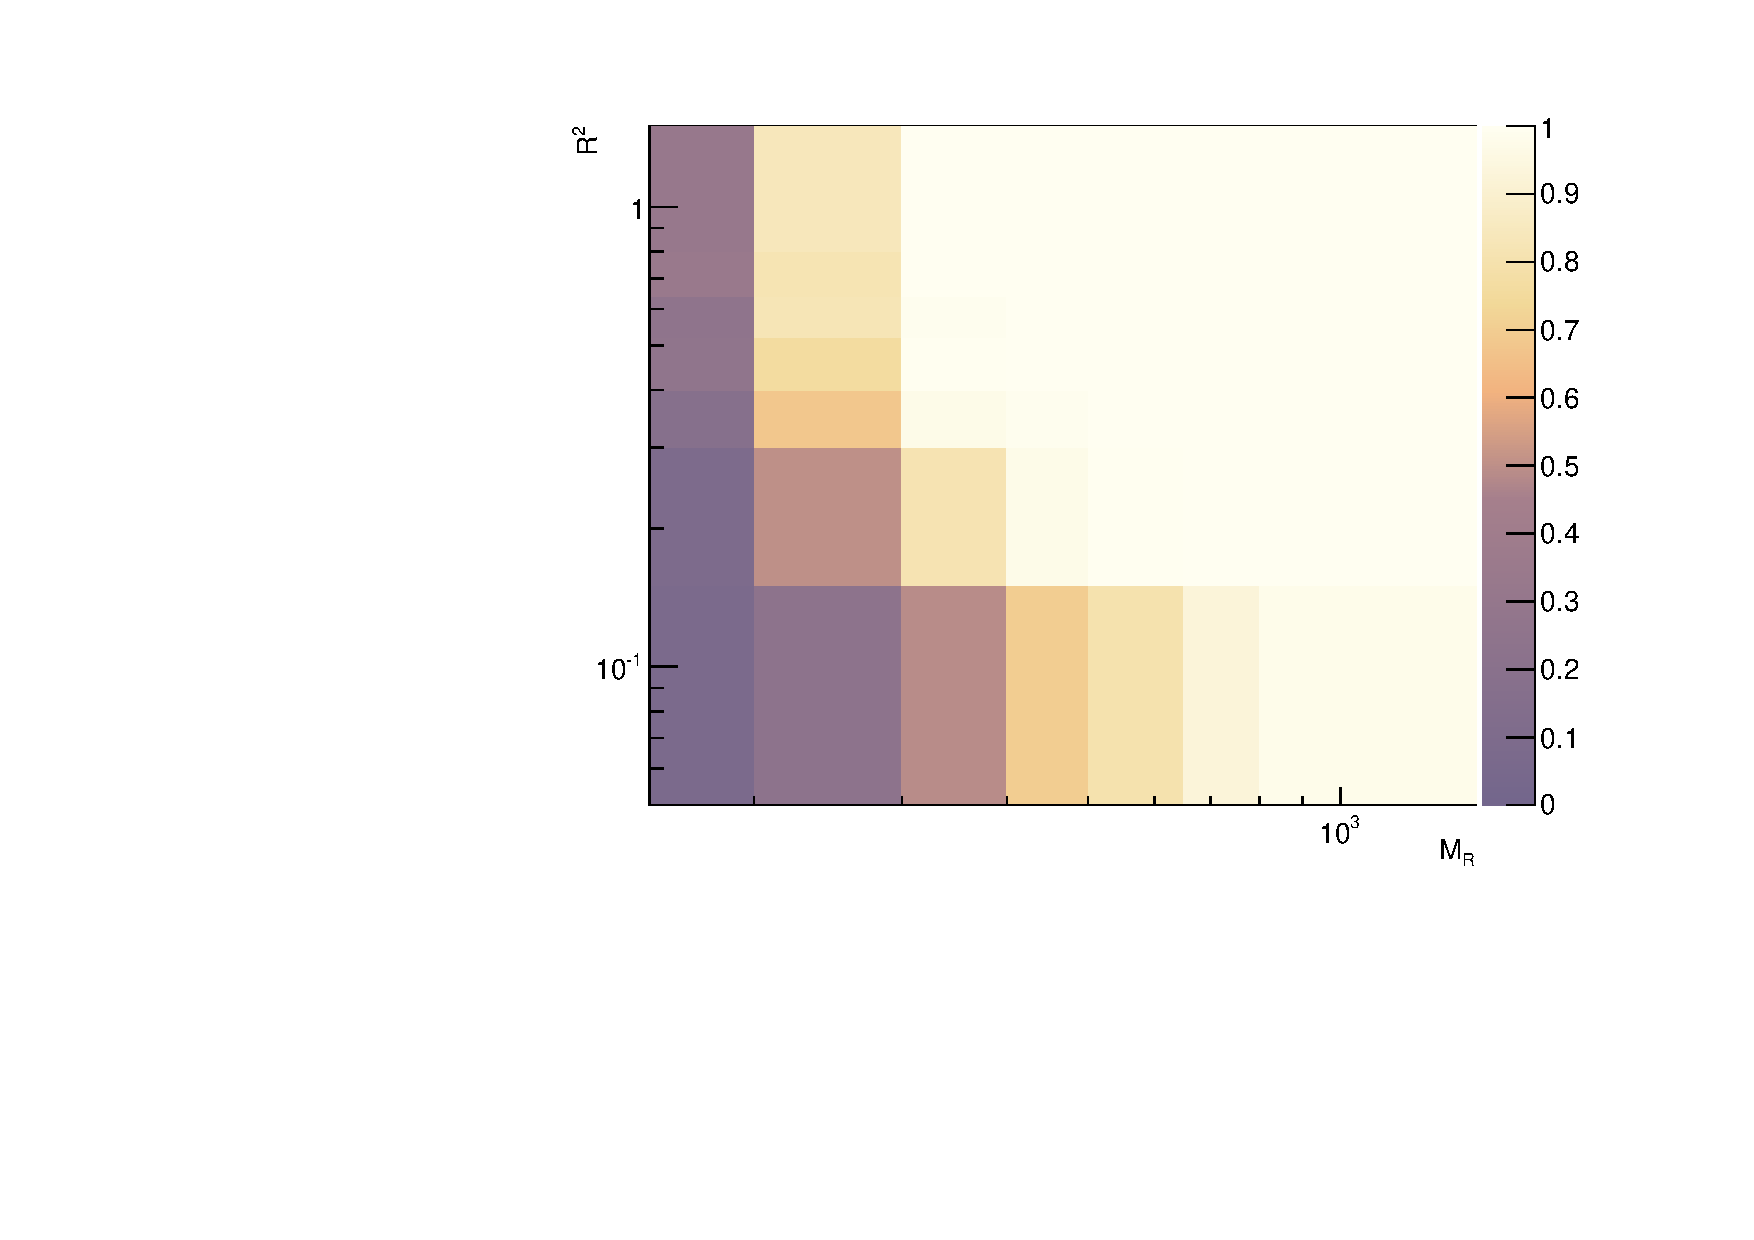
\includegraphics[width=0.45\textwidth]{ht130_MHT_HT_0_3_OR_ht200_file2.pdf}
\caption{\label{fig:at} 2D binned plot in efficiencies for $M_R$ and $R_2$ in T2qq with squark mass of 450 GeV and LSP mass of 400 GeV, with $H_T>200$ GeV OR  $H_T>130$ GeV \& $H_T^{miss}/H_T >$ 0.3. The z color axis refers to the efficiency.}
\end{figure}
\begin{figure}
 %\centering
 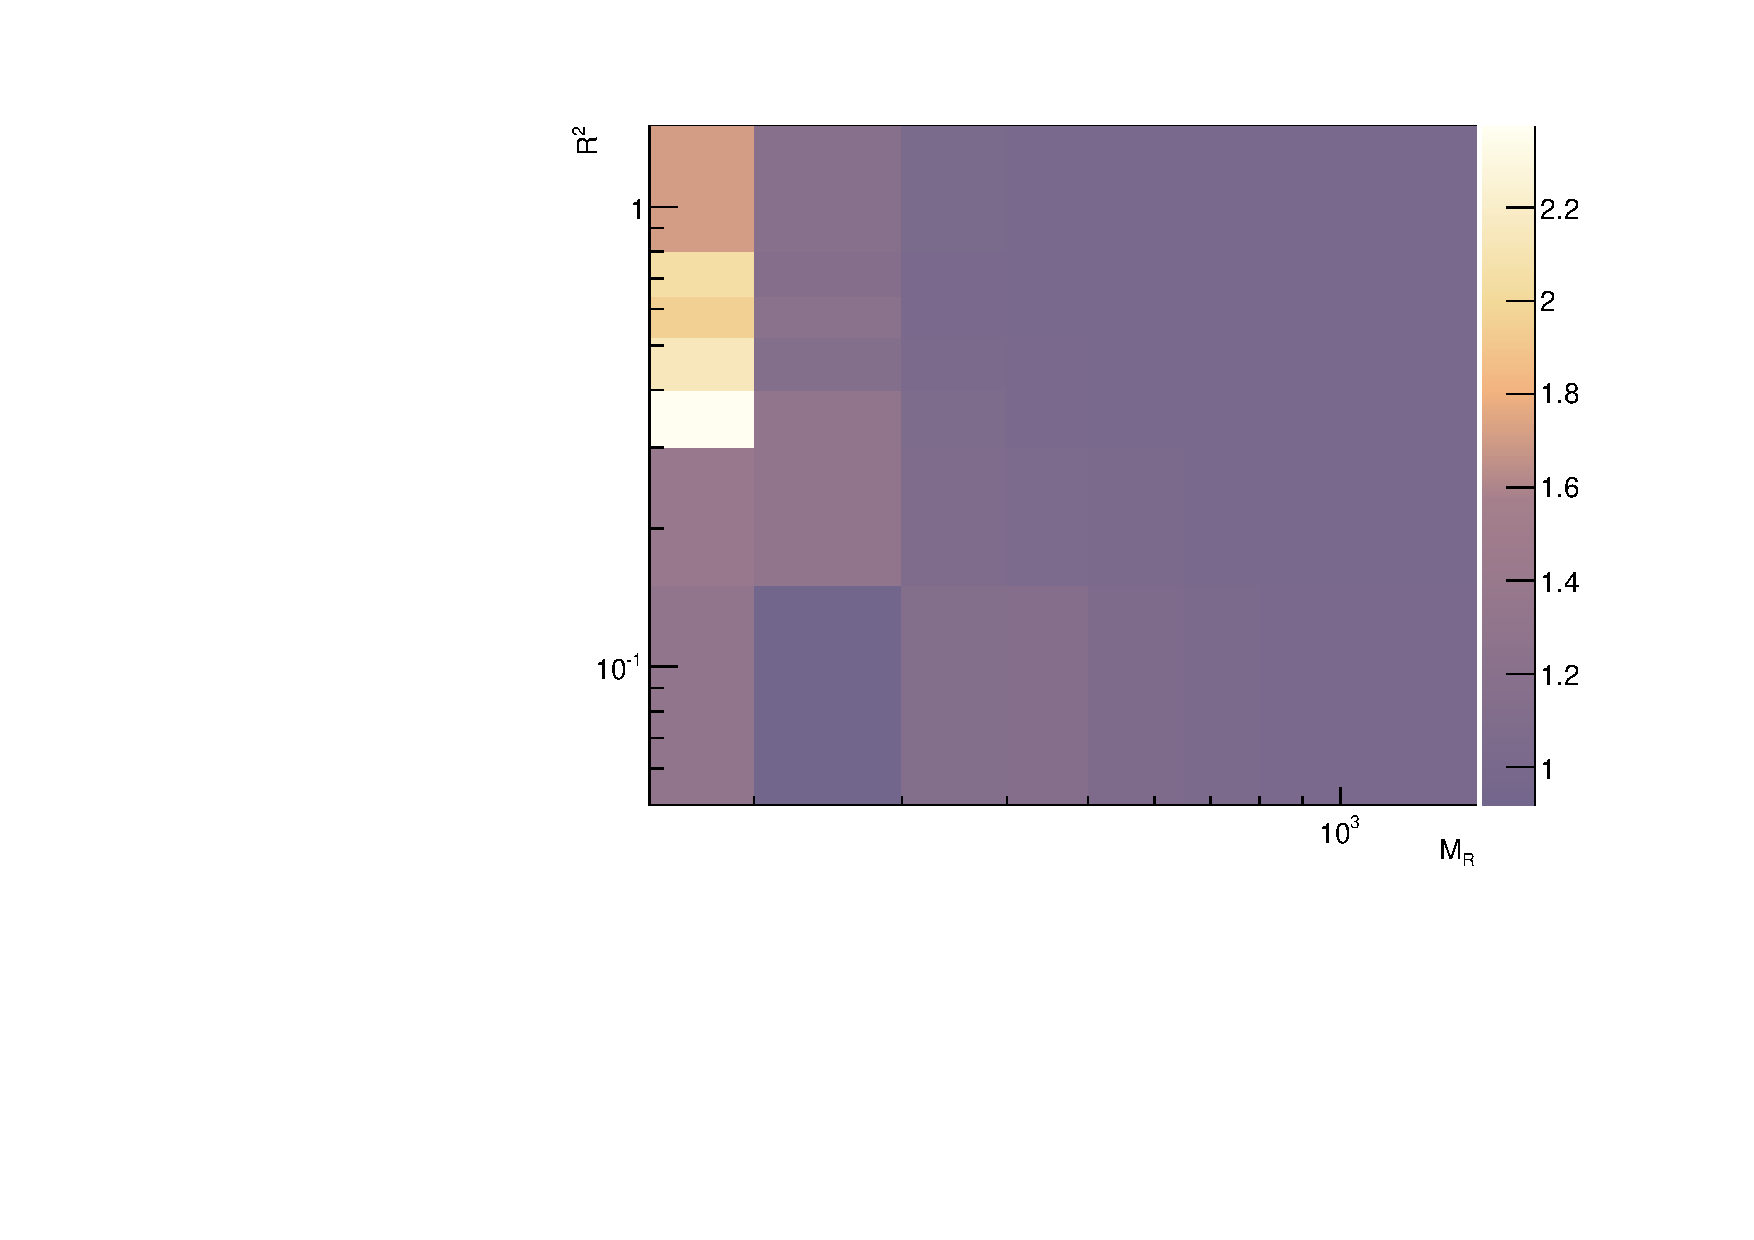
\includegraphics[width=0.45\textwidth]{ratio_MHTHT_vs_new_trigger_file2.pdf}
\caption{\label{fig:ratio_at} 2D binned plot of the ratio of events for $M_R$ and $R_2$ in T2qq with squark mass of 450 GeV and LSP mass of 400 GeV, with a numerator of $H_T>200$ GeV OR  $H_T>130$ GeV \& $H_T^{miss}/H_T >$ 0.3, and a denominator of $H_T>200$ GeV OR  $H_T>125$ GeV \& single jet $p_T>120$ \& two jets with $p_T>30$ \& $\Delta\phi<$2.6 radians. The z color axis refers to the ratio.}
\end{figure}
\begin{figure}
 %\centering
 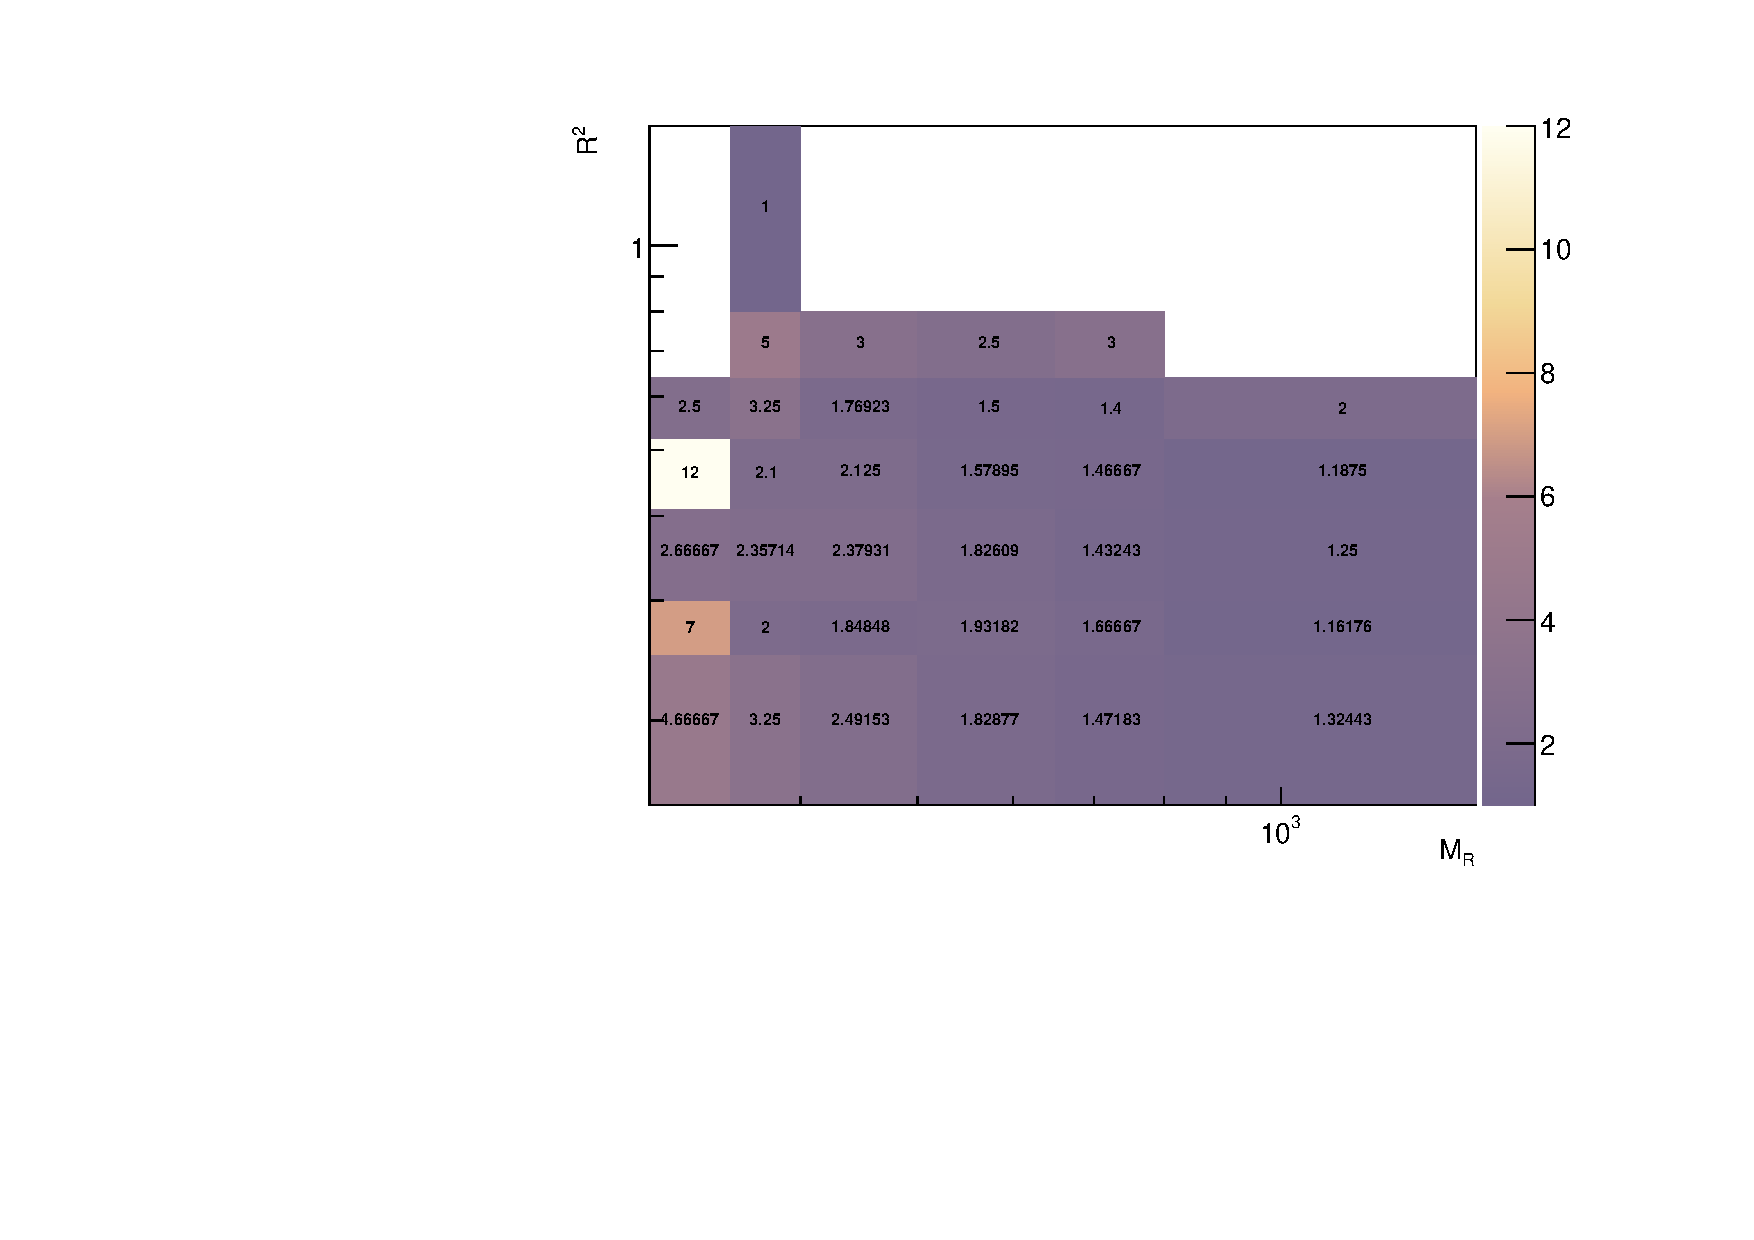
\includegraphics[width=0.45\textwidth]{RATIOquad_ht150_quadcenjet_30_file8.pdf}
\caption{\label{fig:ratio} 2D binned plot of the ratio of events for $M_R$ and $R_2$ in T1qqqq with gluino mass of 800 GeV and LSP mass of 575 GeV, with a numerator of $H_T>150$ GeV and quadjet $p_{T} >$ 30 GeV, and a denominator of quadjet $p_T >$ 60 GeV. The z color axis refers to the ratio.}
\end{figure}
\begin{figure*}
 %\centering
 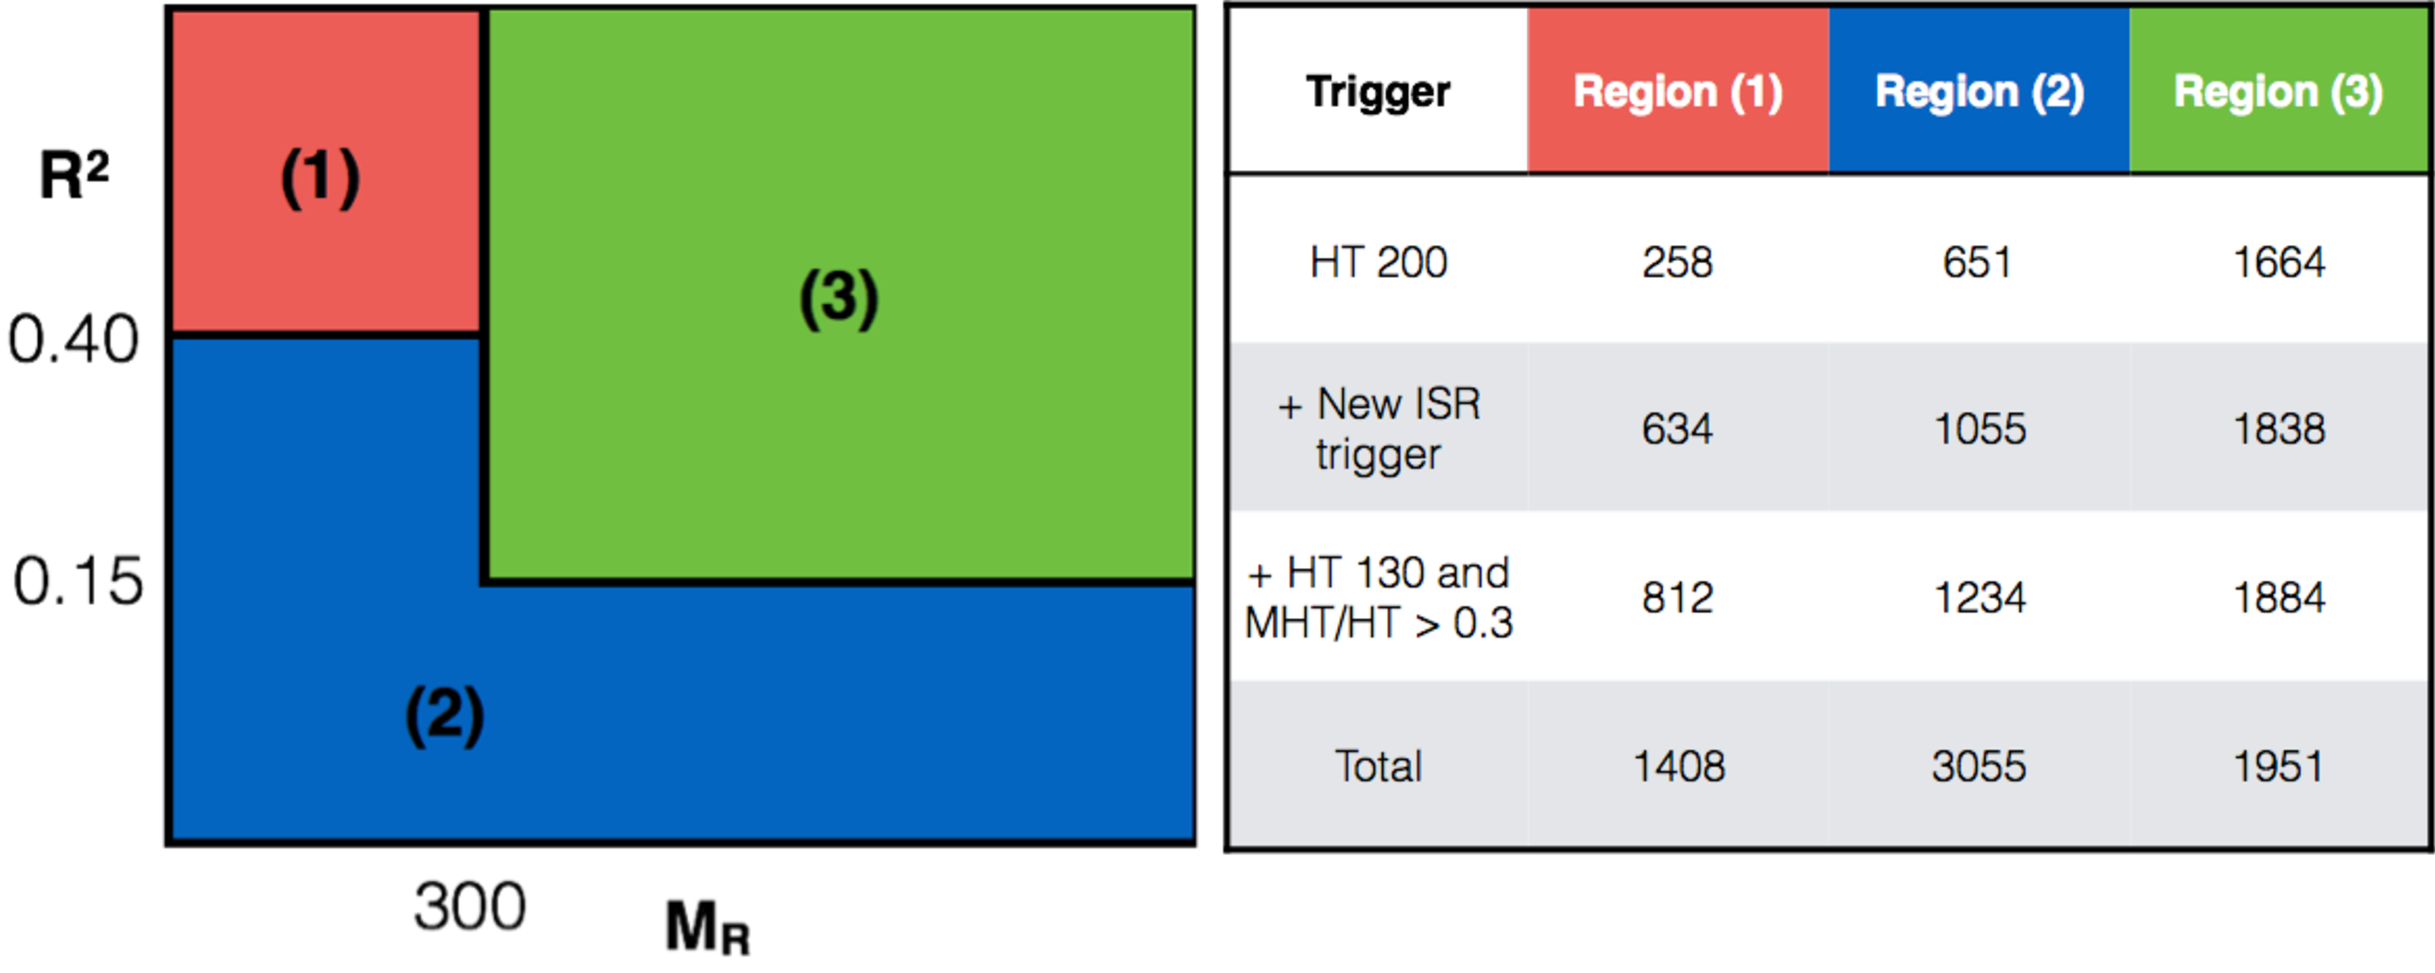
\includegraphics[width=0.98\textwidth]{eff_figure.pdf}
\caption{\label{fig:region} Regions of comparison for the hadronic triggers in the $M_R$, $R^2$ plane from 150 to 1400 GeV in $M_R$ and 0.05 to 1.5 in $R^2$. Events passing the selection in each region were recorded in the table on the right. All additional triggers are examined with the OR of $H_T >$ 200 GeV. These numbers are for the T2qq sample with a squark mass of 450 GeV and an LSP mass of 400 GeV.}
\end{figure*}
\section{Level 1}
\subsection{Methods}
Several variations of hadronic L1 triggers were investigated. We looked at a few forms of the $H_T$ trigger. At the L1 level, $H_T$ is calculated as the sum of the $E_T$s of the 4x4 trigger towers \cite{ucsb}.  These regions are each defined in azimuthal by $20^{\circ}$ in the azimuthal angle $\phi$, with divisions in psuedorapidity $\eta$ as well \cite{hlt}. To investigate the relationship between the razor variables and this trigger, two dimensional binned efficiency plots in generator-level $M_{R}$ and $R^2$ were created with different selections on L1 data. In general, the baseline selection included a calorimeter region transverse energy $E_T$ threshold of 7 GeV, with an $|\eta| <$  3, or a jet $p_T$ minimum of 10 GeV if jet selection was involved. For single jet studies, we only had a baseline jet minimum. The datasets for which these efficiencies were calculated included $t\bar{t}$+jets, which is a common Standard Model background for SUSY searches, as well as the SUSY signals T2tt and T2qq. T2qq refers to first and second generation squark-antisquark production, decaying to quark/antiquark and two LSPs. T2tt refers to stop/antistop pair production, decaying to top/antitop and two LSPs. The T2tt sample had $m_{\tilde{t}}=800$ GeV and $m_{\tilde{\chi}^0_1}=100$ GeV, and the T2qq samples had $m_{\tilde{q}}=400$ GeV and $m_{\tilde{\chi}^0_1}=150$ GeV, $m_{\tilde{q}}=450$ GeV and $m_{\tilde{\chi}^0_1}=400$ GeV, and $m_{\tilde{q}}=600$ GeV and $m_{\tilde{\chi}^0_1}=100$ GeV. We also investigated a T1qqqq sample for our quadjet studies and our jet algorithm studies, which refers to gluino pair production decaying to four quarks and two LSPs. A summary of the pair-produced particles and their decay products can be found in Table \ref{table:signals}. The SUSY signal samples were generated by Maria D'Alfonso from UCSB \cite{ucsb}. 
\subsection{Results}
\par $H_T$ cuts over a broad range of energies were examined. In figure 5, the efficiency over a region of $M_R$ and $R_2$ from 400 to 1450 GeV in $M_R$ and 0.25 to 1.5 in $R^2$ was plotted for increasing cuts in GeV. We see here that all samples drop to efficiency below 0.95 after the $H_T$ selection is greater than 210-220 GeV. We aim to keep efficiencies above 0.95 because low efficiencies pose a problem for fits later on in the razor analyses \cite{talk}. If we look lower in $M_R$ and $R^2$, we can see that the efficiency drops for low $M_R$ (Fig. \ref{fig:eff_t2tt}-\ref{fig:eff_t2com}).  
\par The addition of a $\Delta \phi$ cut was also examined for 2.6 radians. This is motivated by the trend that quantum chromodynamics (QCD) background mostly lies at high $\Delta \phi$, where $\Delta \phi$ is the azimuthal angle difference between any two jets. To minimize the rate of this new trigger while selecting for events lower in $H_T$, members of the CMS internal SUSY Group proposed this cut with the added criteria of a leading jet $p_T$ cut of 120 GeV as well as a subleading jet $p_T$ cut of 30 GeV \cite{susy_group}. With the addition of this trigger, we see a marked improvement in lower $M_R$ (Fig. \ref{fig:eff_t2com}, \ref{fig:comp}).
\par An alternate trigger was proposed by the CMS internal SUSY Group that involves selection on $H_T^{miss}$ values, which is defined as the negative vectorial sum of the region $E_T$ values \cite{susy_group}. The trigger requires $H_T > 130$ GeV in conjunction with $H_T^{miss}/H_T >$ 0.3 to keep rates low. This improves on the previously mentioned trigger with the angle cut (Fig. \ref{fig:at}, \ref{fig:ratio_at}). To fully evaluate the usefulness of these two proposed triggers, events passing certain regions in the $M_R$,$R^2$ plane were directly compared (Fig. \ref{fig:region}). The $H_T^{miss}$ has a noticeable improvement in region I of low $M_R$, high $R^2$, an area which is particularly important for dark matter searches \cite{dark_razor}.
\begin{figure}[h]
 %\centering
 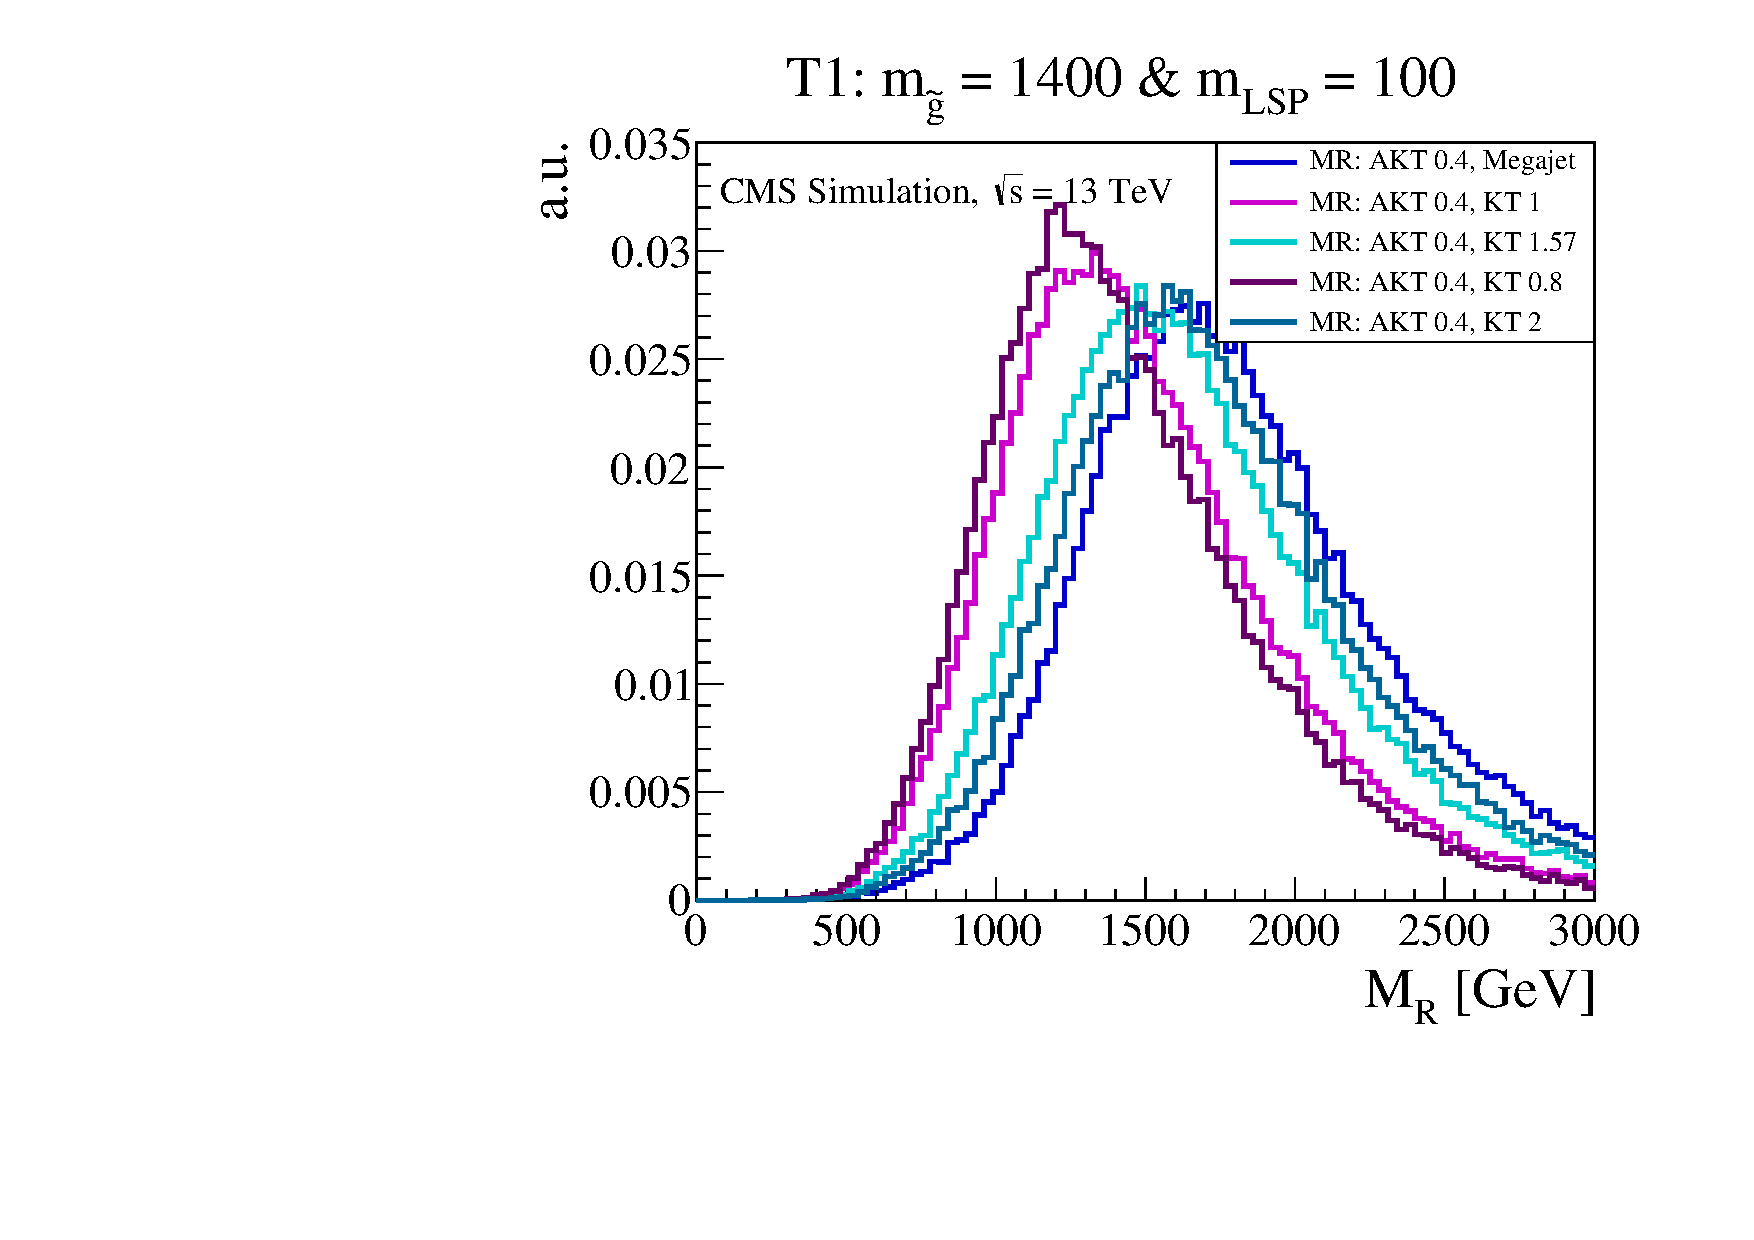
\includegraphics[width=0.45\textwidth]{cones_T1_1400_100_0_4.pdf}
\caption{\label{fig:t1_clstr} $M_R$ distributions of T1 for anti-$k_T$ inclusive jets, which are then clustered with either the megajet algorithm or the $k_T$ algorithm, using various cone sizes. The legend numbers specify the cone size.}
\end{figure}
\begin{figure}[h]
 %\centering
 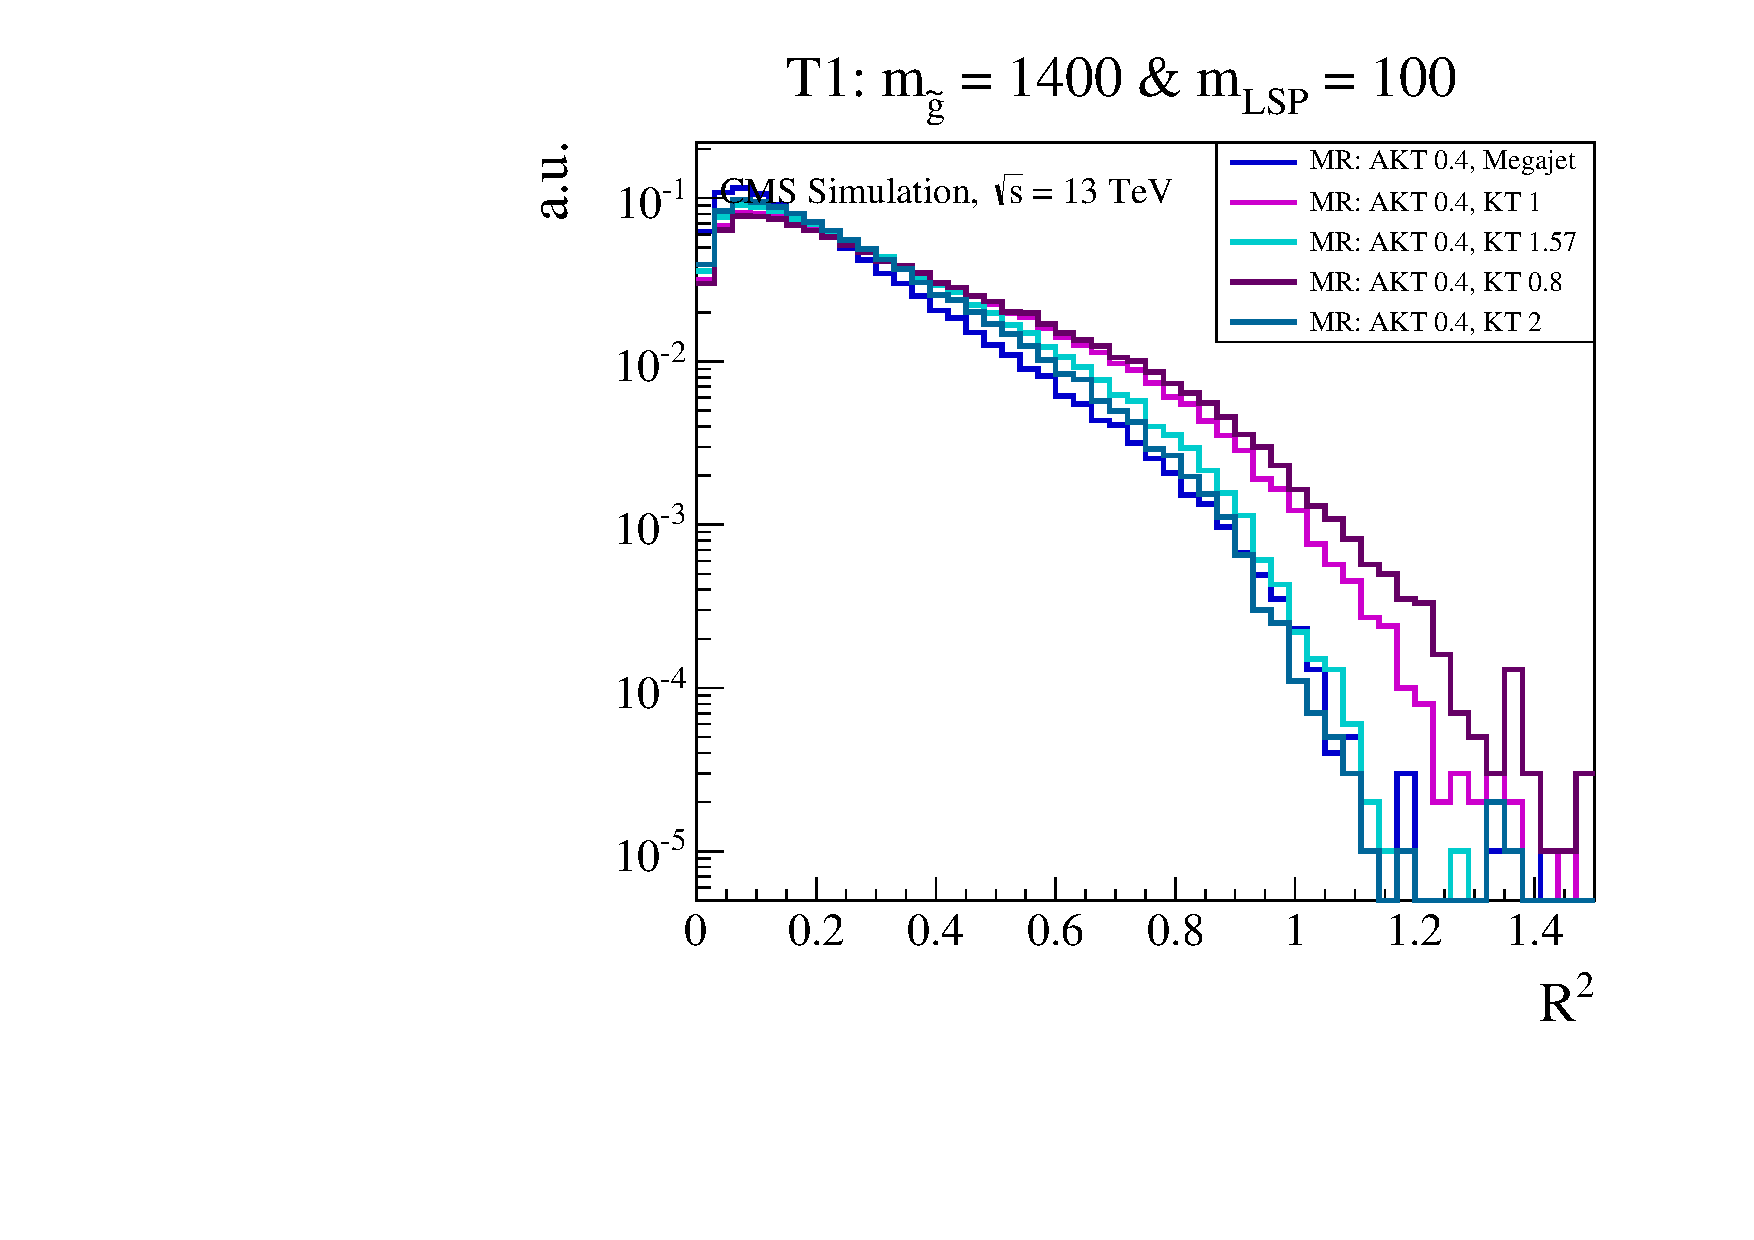
\includegraphics[width=0.45\textwidth]{r2_cones_T1_1400_100_0_4.pdf}
\caption{\label{fig:t1_clstr_r2} $R^2$ distributions of T1 for anti-$k_T$ inclusive jets, which are then clustered with either the megajet algorithm or the $k_T$ algorithm, using various cone sizes. The legend numbers specify the cone size. }
\end{figure}
\begin{figure}
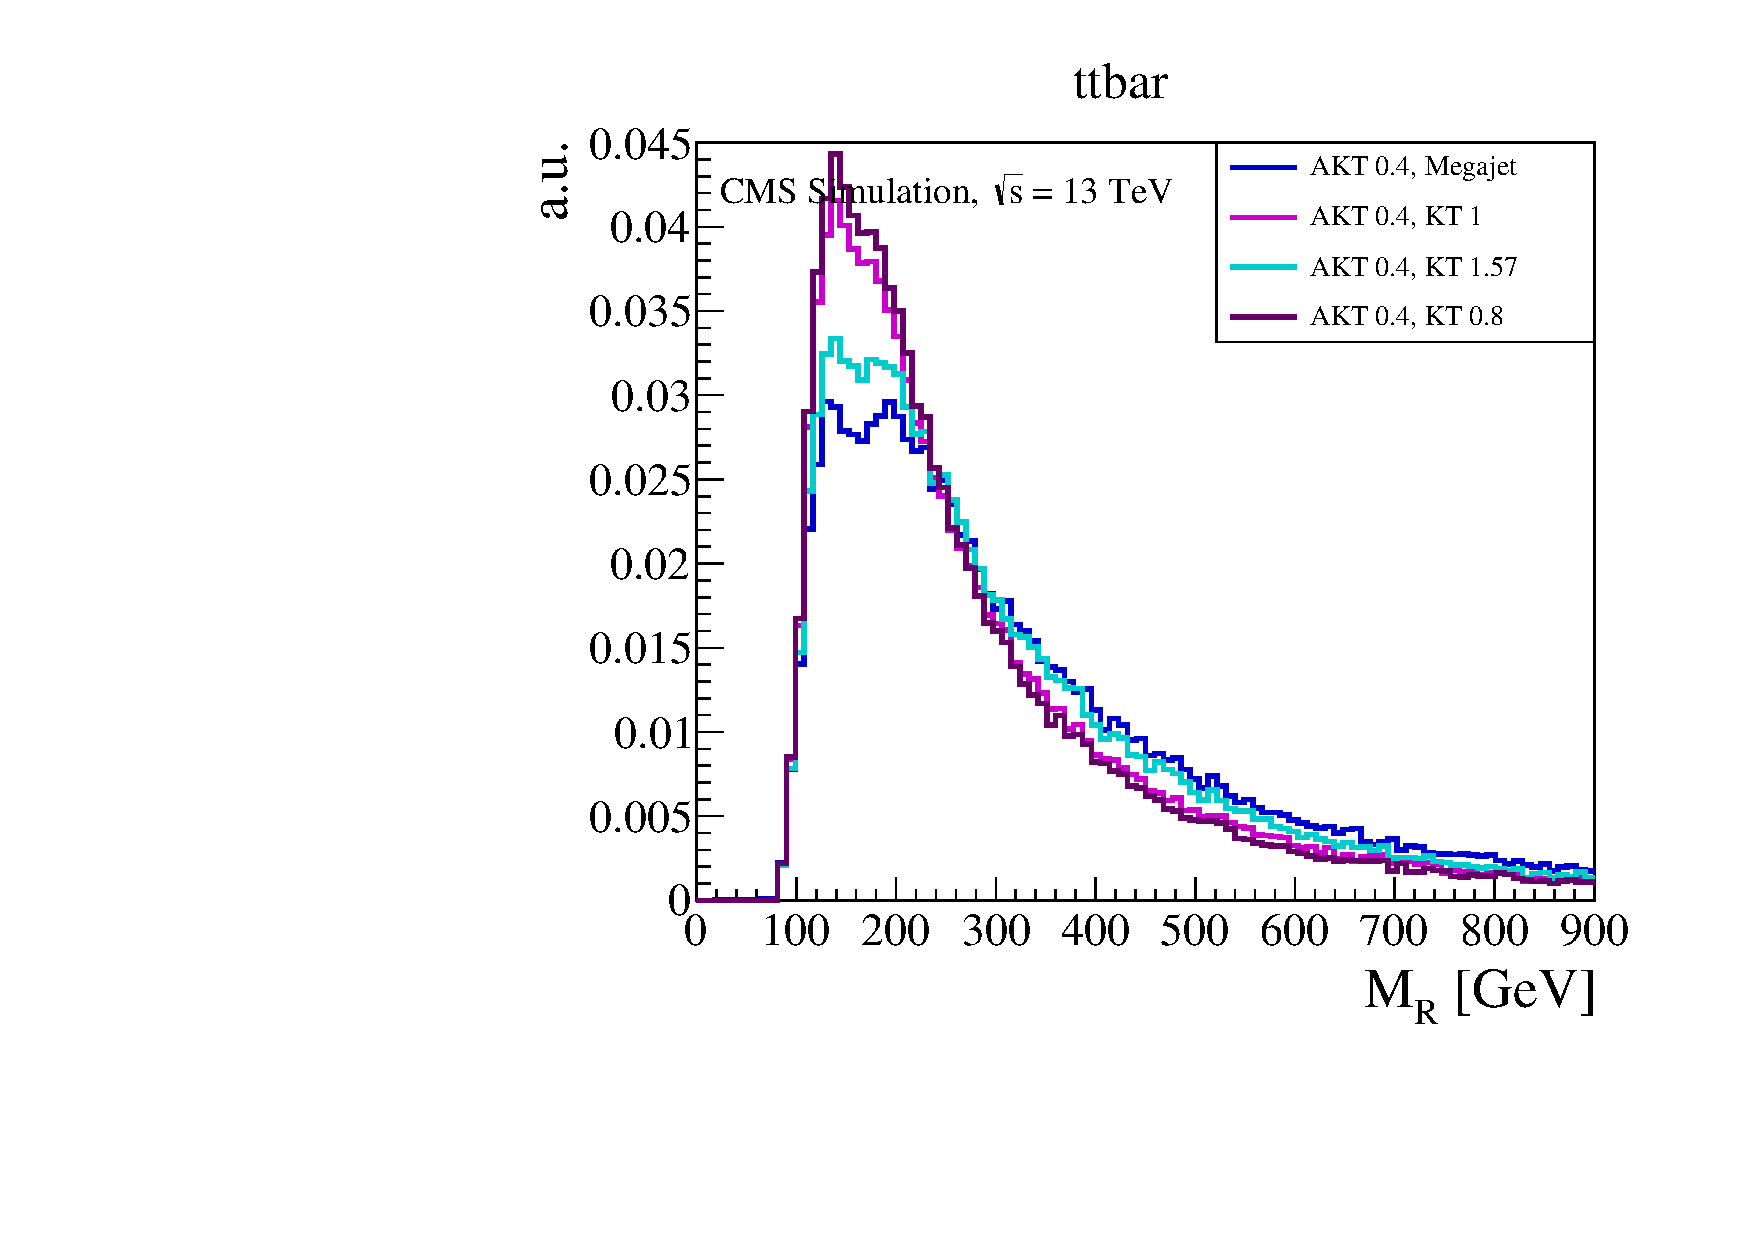
\includegraphics[width=0.45\textwidth]{cones_ttbar_0_4.pdf}
\caption{\label{fig:ttbar_clstr} $M_R$ distributions of $t\bar{t}$+jets for anti-$k_T$ inclusive jets, which are then clustered with either the megajet algorithm or the $k_T$-exclusive algorithm, using various jet radii. }
\end{figure}
\begin{figure}
 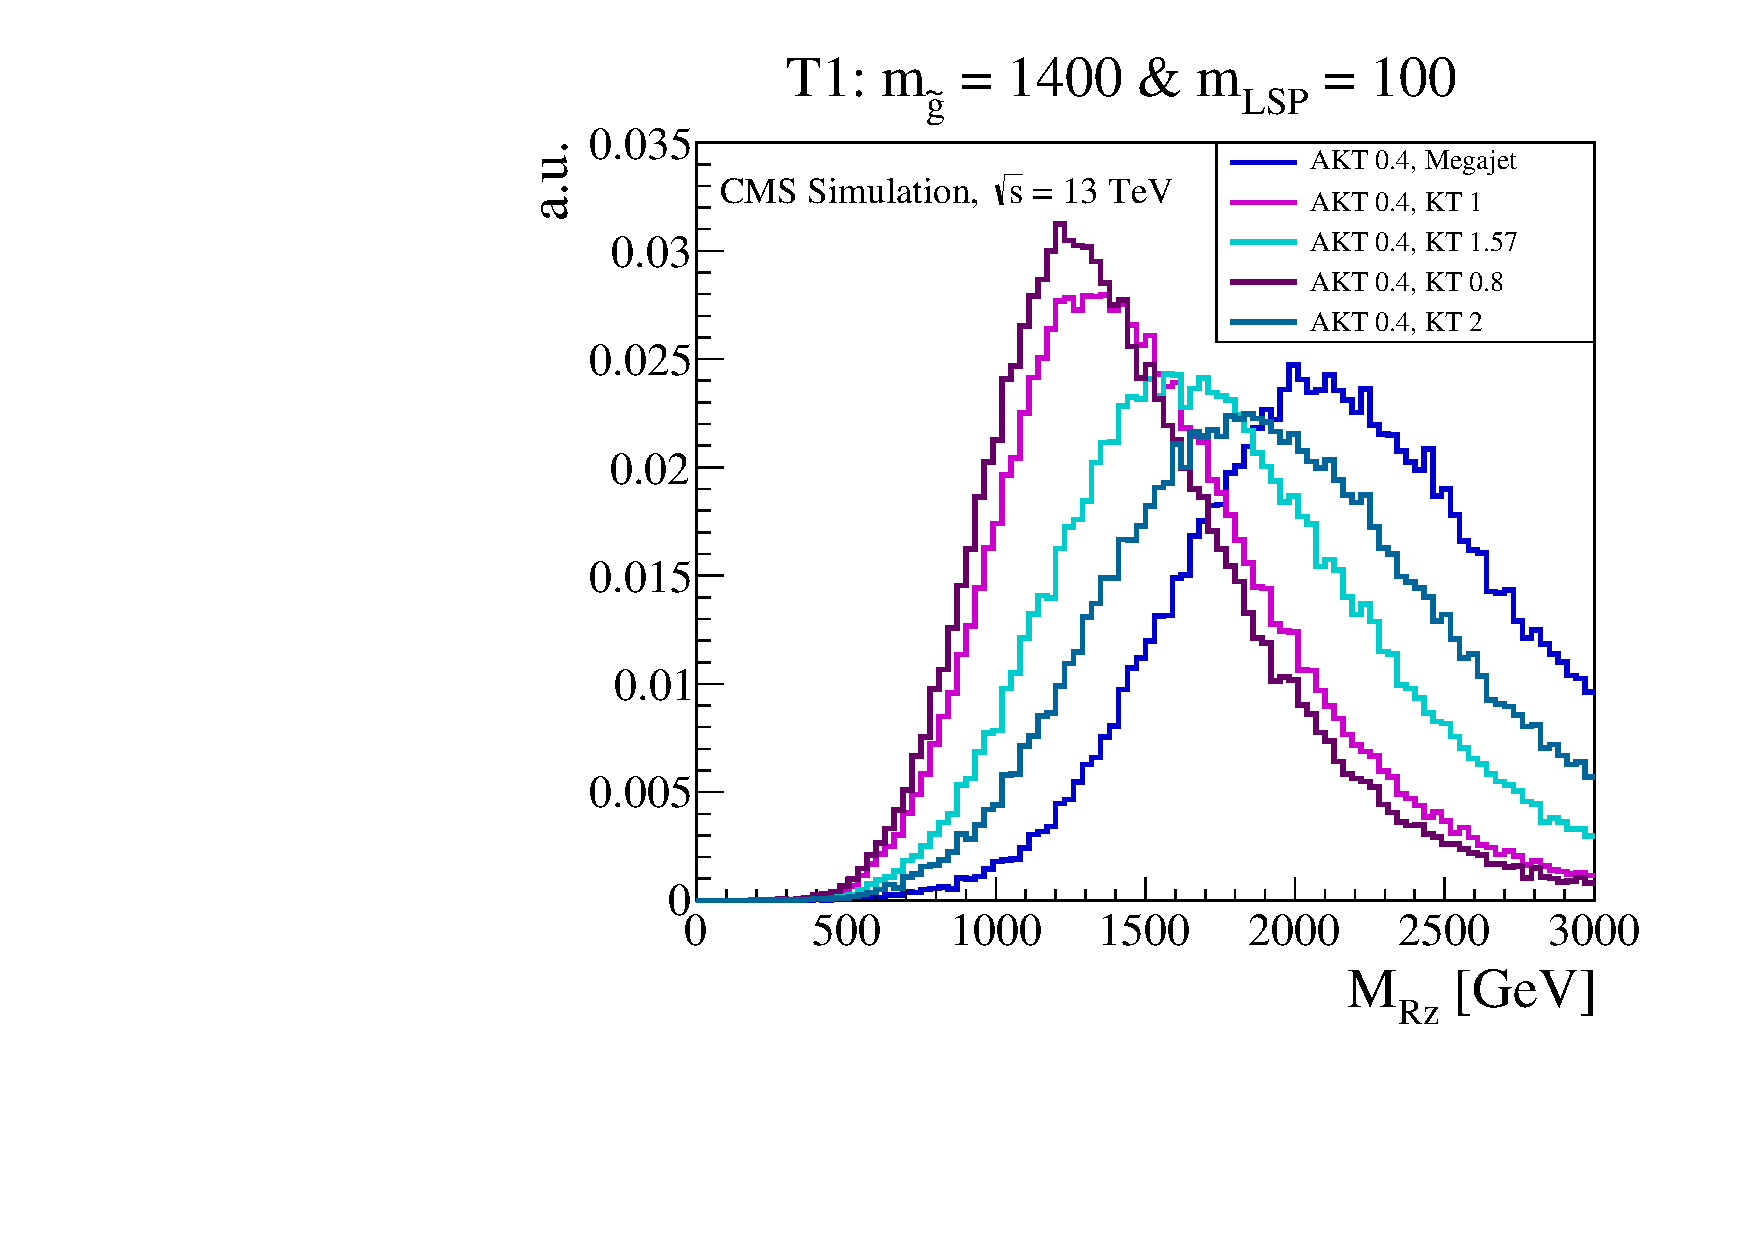
\includegraphics[width=0.45\textwidth]{z_cones_T1_1400_100_0_4.pdf}
\caption{\label{fig:t1_zclstr} $M_{Rz}$ distributions of T1 for anti-$k_T$ inclusive jets, which are then clustered with either the megajet algorithm or the $k_T$-exclusive algorithm, using various jet radii. }
\end{figure}
\begin{figure}
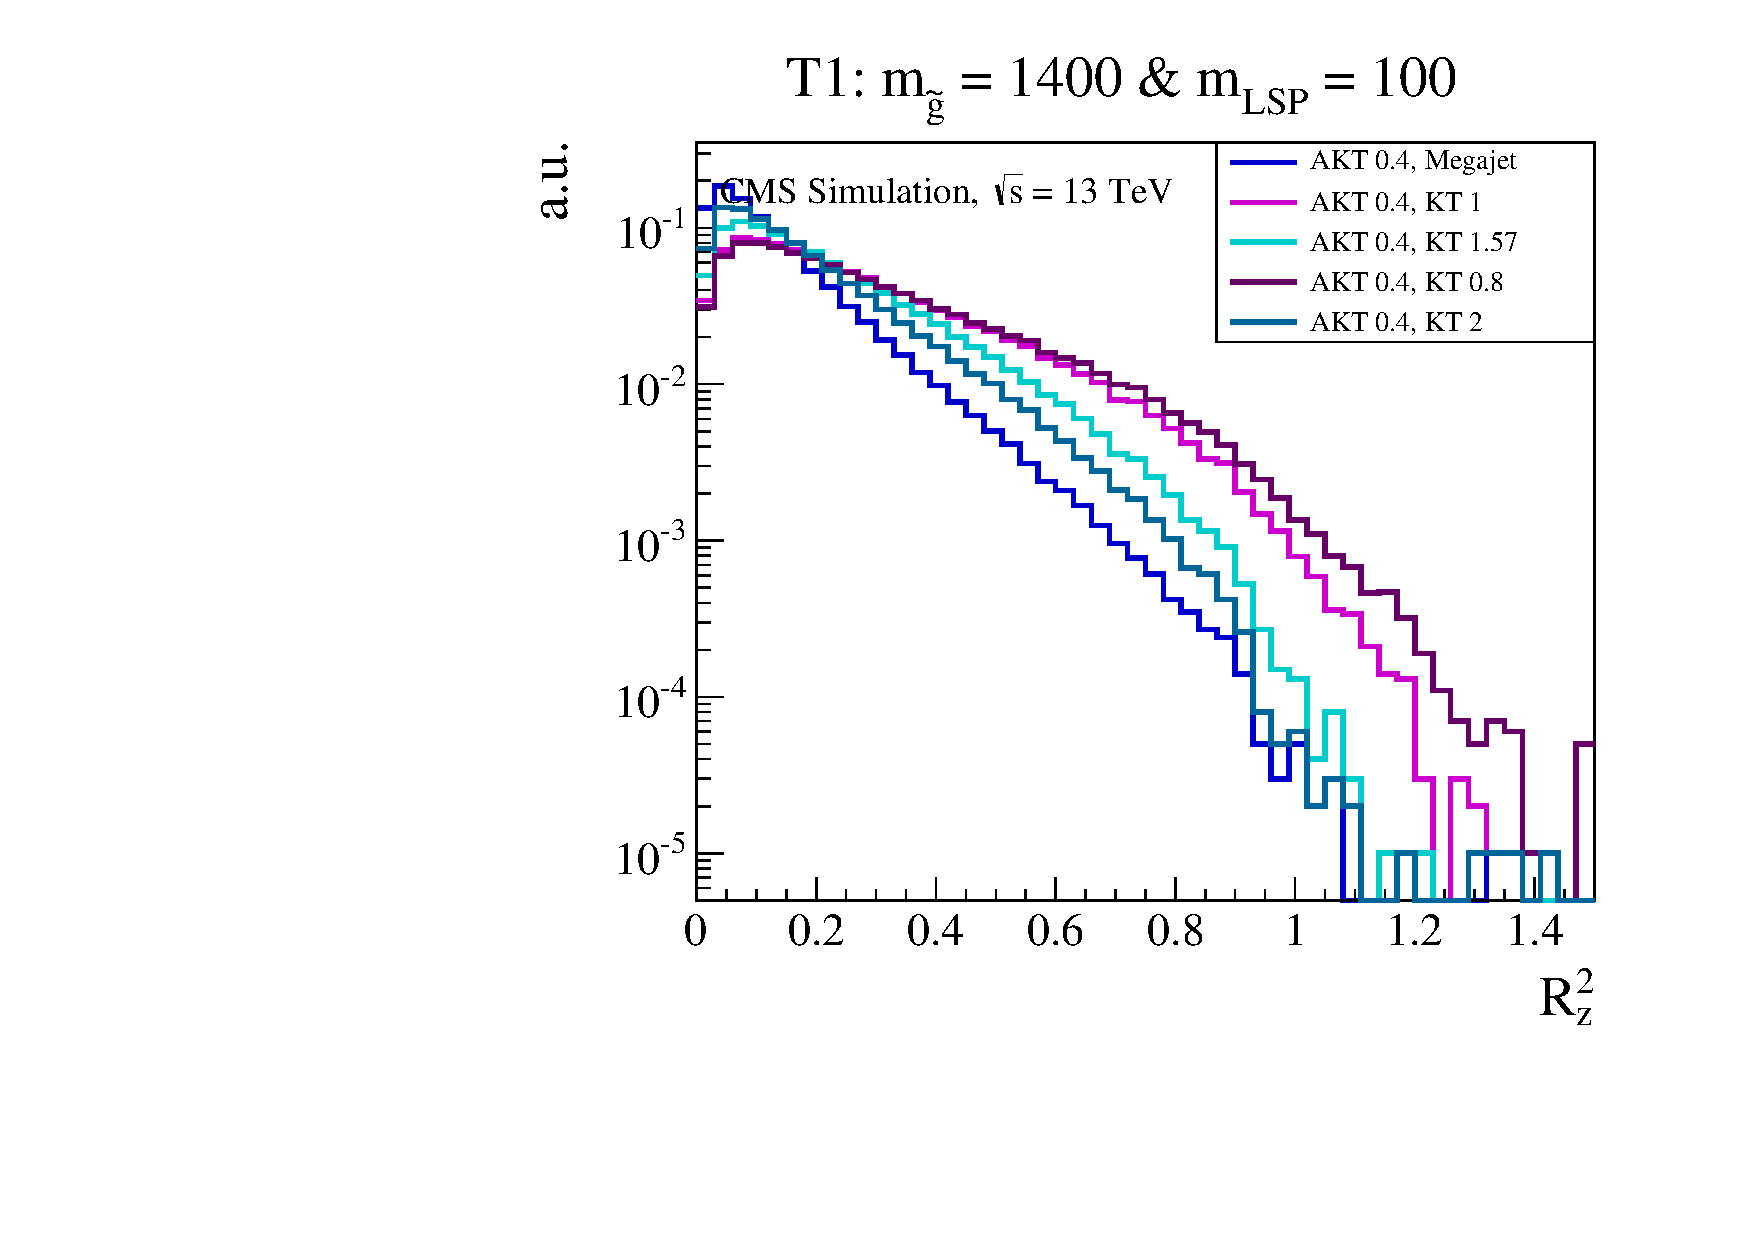
\includegraphics[width=0.45\textwidth]{z_r2_cones_T1_1400_100_0_4.pdf}
\caption{\label{fig:t1_zclstr_r2} $R^2_z$ distributions of T1 for anti-$k_T$ inclusive jets, which are then clustered with either the megajet algorithm or the $k_T$-exclusive algorithm, using various jet radii. }
\end{figure}
\begin{figure}
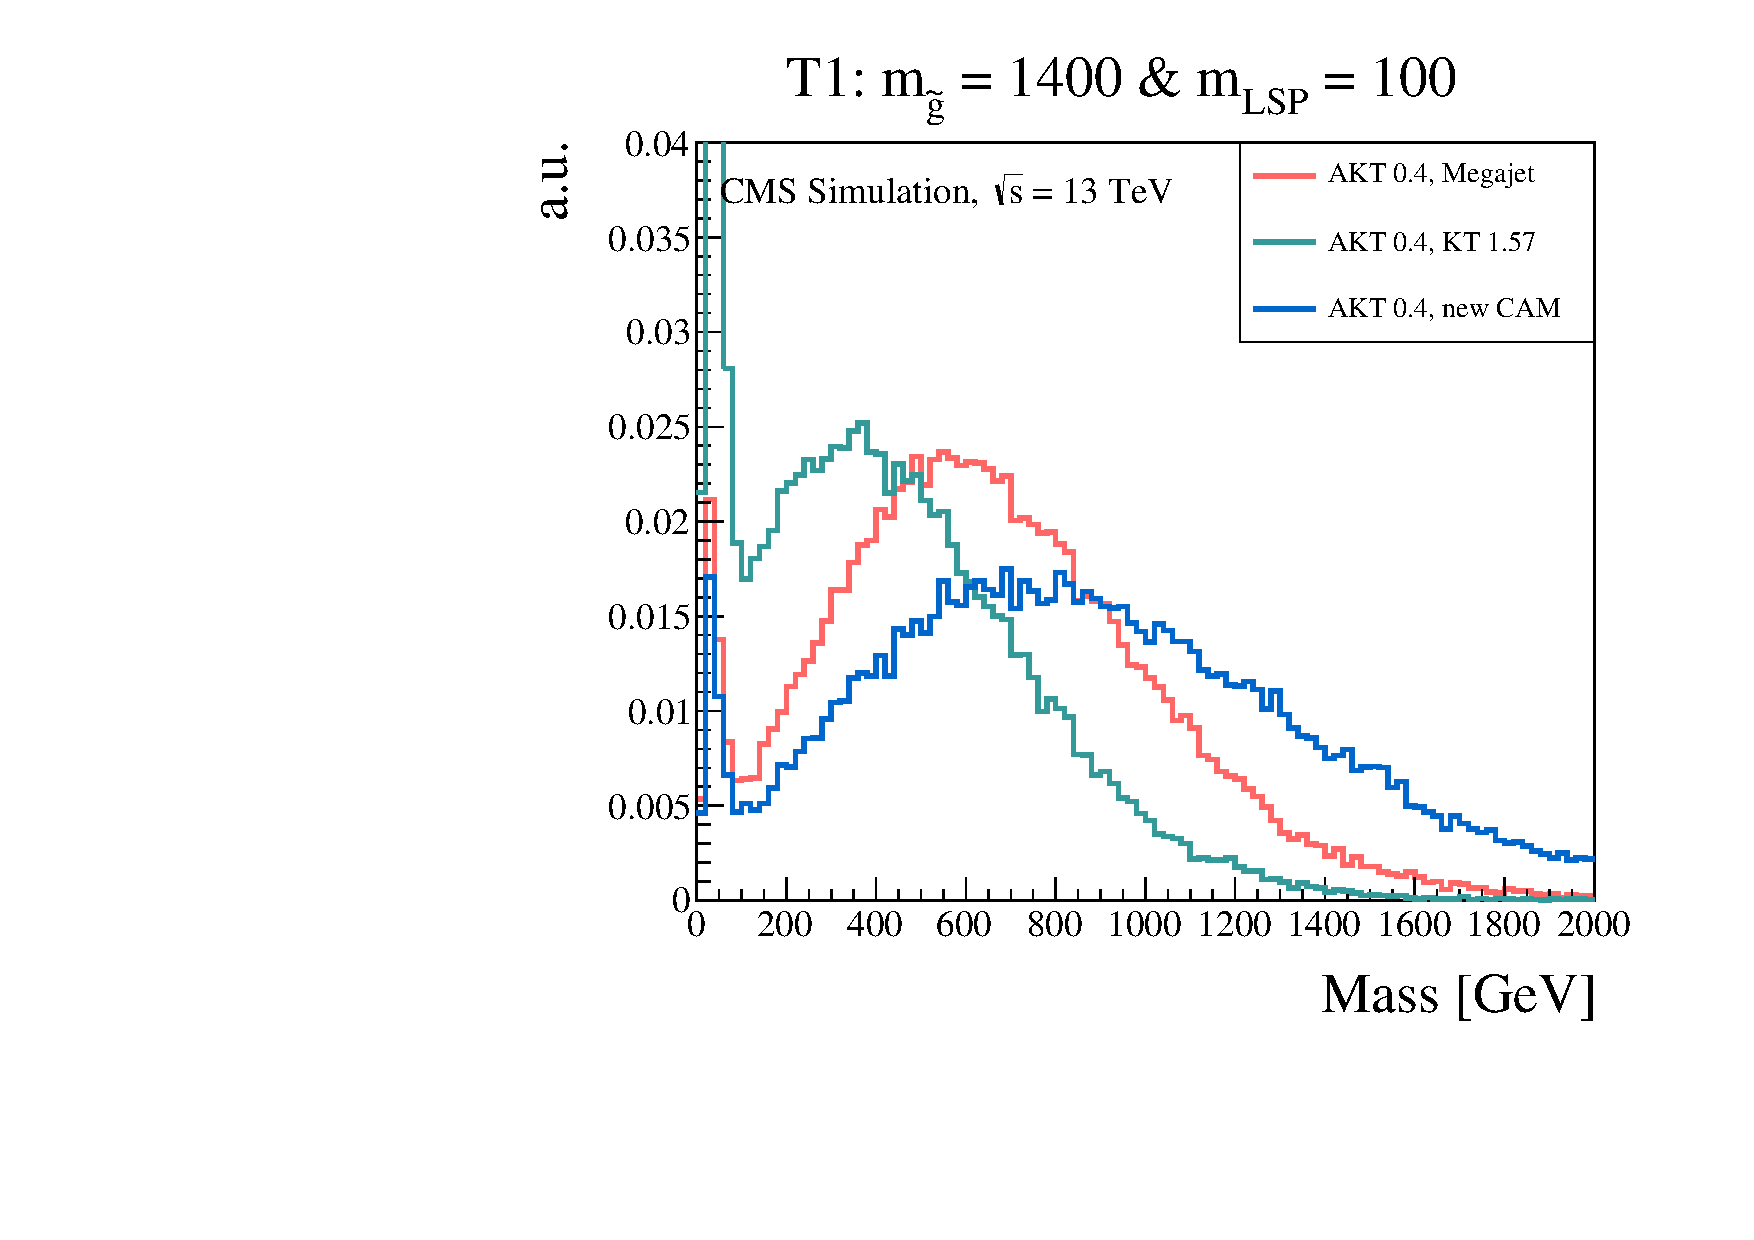
\includegraphics[width=0.45\textwidth]{T1_1400_100_new_masses.pdf}
\caption{\label{fig:t1_masses} Mass distributions of the $p_T$-leading hemisphere T1 for anti-$k_T$ inclusive jets that are clustered with the megajet algorithm, the $k_T$-exclusive algorithm, or the new clustering algorithm. }
\end{figure}
\par We can also look at alternatives to the quadjet trigger. Since the currently proposed quadjet trigger cuts on a $p_T$ value of greater than 60 GeV, we suggest an replacement trigger of $H_T > 175$ GeV and a quadjet $p_{T}$ cut of 30 GeV. $H_T$ involves a sum, which will allow for jets of lower $p_{T}$ to pass the trigger. As a result, we see a recovery of events for the $M_R$ and $R^2$ plane (Fig. \ref{fig:ratio}).
\section{High Level Trigger}
\subsection{Methods}
HLT objects involve more reconstruction, and involve software triggers rather than hardware triggers \cite{hlt}. The events selected for at L1 are grouped into categories (i.e. two jets with $p_{T} >$  100 GeV), and these categories feed into the HLT. For the razor searches, we need HLT triggers that select for events that pass a certain $M_R$ or $R^2$ cut. However, the reconstruction of these $M_R$ and $R^2$ values is nontrivial. For an all-hadronic razor analysis, $M_R$ and $R^2$ are constructed using two hemispheres of hadronic jets. Jets originate from the hadronization of quarks and gluons. The origin of the final state of the hadrons is determined using a clustering scheme. There are several clustering schemes in common use which include anti-$k_T$, $k_T$, and Cambridge \cite{fastjet}. These schemes depend on a metric called jet radius, which is defined as $\Delta R^2 = \Delta\eta^2+\Delta\phi^2$, where $\eta$ is rapidity and $\phi$ is the azimuthal angle.
\par At the HLT, we receive jets as an inclusively anti-$k_T$ clustered set, which we then cluster to form two hemispheres of jets. The precedent for the razor analysis is to use megajet clustering, which involves minimizing the sum of the invariant masses of the two hemispheres in quadrature, which contains relevant angle information if we assume that the hemispheres are approximately massless \cite{talk}. Here, we investigate this algorithm, as well as the $k_T$ algorithm with various cone sizes, in using the built-in exclusive method to form hemispheres. Details on this method as well as the differences between inclusive and exclusive clustering have been previously studied \cite{fastjet} . A preliminary investigation into a new jet clustering algorithm is also conducted. This new algorithm clusters jets inclusively using the Cambridge scheme with increasing jet radius until there are two clustered hemispheres remaining. Generator-level Monte Carlo data was created using the PYTHIA software \cite{pythia}. We investigate two signal models: T1qqqq and T2qq with $t\bar{t}$+jets background.
%MOVE FIGURES BACK HERE
\subsection{Results}
Jet radius has a visible effect on both $M_R$ and $R^{2}$. We see the most obvious effect in T1qqqq (gluino mass = 1400 GeV, LSP mass = 100 GeV), probably due to the higher number of jets. With increasing jet radius R, the $M_R$ peak is pushed towards larger values and broadened (Fig \ref{fig:t1_clstr}). We also see slightly broader, flatter peaks, which are likely due to the increased number of particles being included with higher jet radius. $R^2$, on the other hand, will fall faster (Fig \ref{fig:t1_clstr_r2}).  For the T2qq signal (quark mass = 500 GeV, LSP mass = 10 GeV) and $t\bar{t}$+jets, similar phenomena can be observed, although to a smaller degree (Fig. \ref{fig:ttbar_clstr}).
\par We also study another $M_R$-like variable, called $M_{Rz}$. Given two hemispheres, we traditionally define $$M_R = \sqrt{(|p^{j1}|+|p^{j2}|)^2-(p_z^{j1}+p_z^{j2})^2}$$ \cite{razor}. Here we investigate a new variable, $M_{Rz}$, which is defined as $$M_{Rz} = \sqrt{(E^{j1}+E^{j2})^2-(p_z^{j1}+p_z^{j2})^2}$$ \cite{talk}. This variable is dependent on the mass of the hemispheres. An increase in KT clustering jet radius increases the number of particles being included in the hemisphere, which may explain the increased dependence on jet radius for the $M_{Rz}$ distributions (Fig. \ref{fig:t1_zclstr}). There is also a dramatic separation of the $R^2_z$ distributions (Fig. \ref{fig:t1_zclstr_r2}). 
\par An initial investigation of the new clustering algorithm proposed reveals that it is physically different from the old clustering algorithm. Since it increases the jet radius until the inclusive clustering results in two jets, it retains all jets. The built-in exclusive clustering, in contrast, will throw away jets of low $p_T$. This is evidenced by the visible increase in hemisphere mass (Fig. \ref{fig:t1_masses}). It also makes dramatically different clustering decisions than the megajet clustering algorithm, as seen in Fig. \ref{fig:eta_phi}. There is a noticeable preference towards clustering jets near one another, while the megajet algorithm's decisions are skewed towards making hemispheres of similar masses. 
\onecolumngrid
\begin{center}
\begin{figure}
\centering
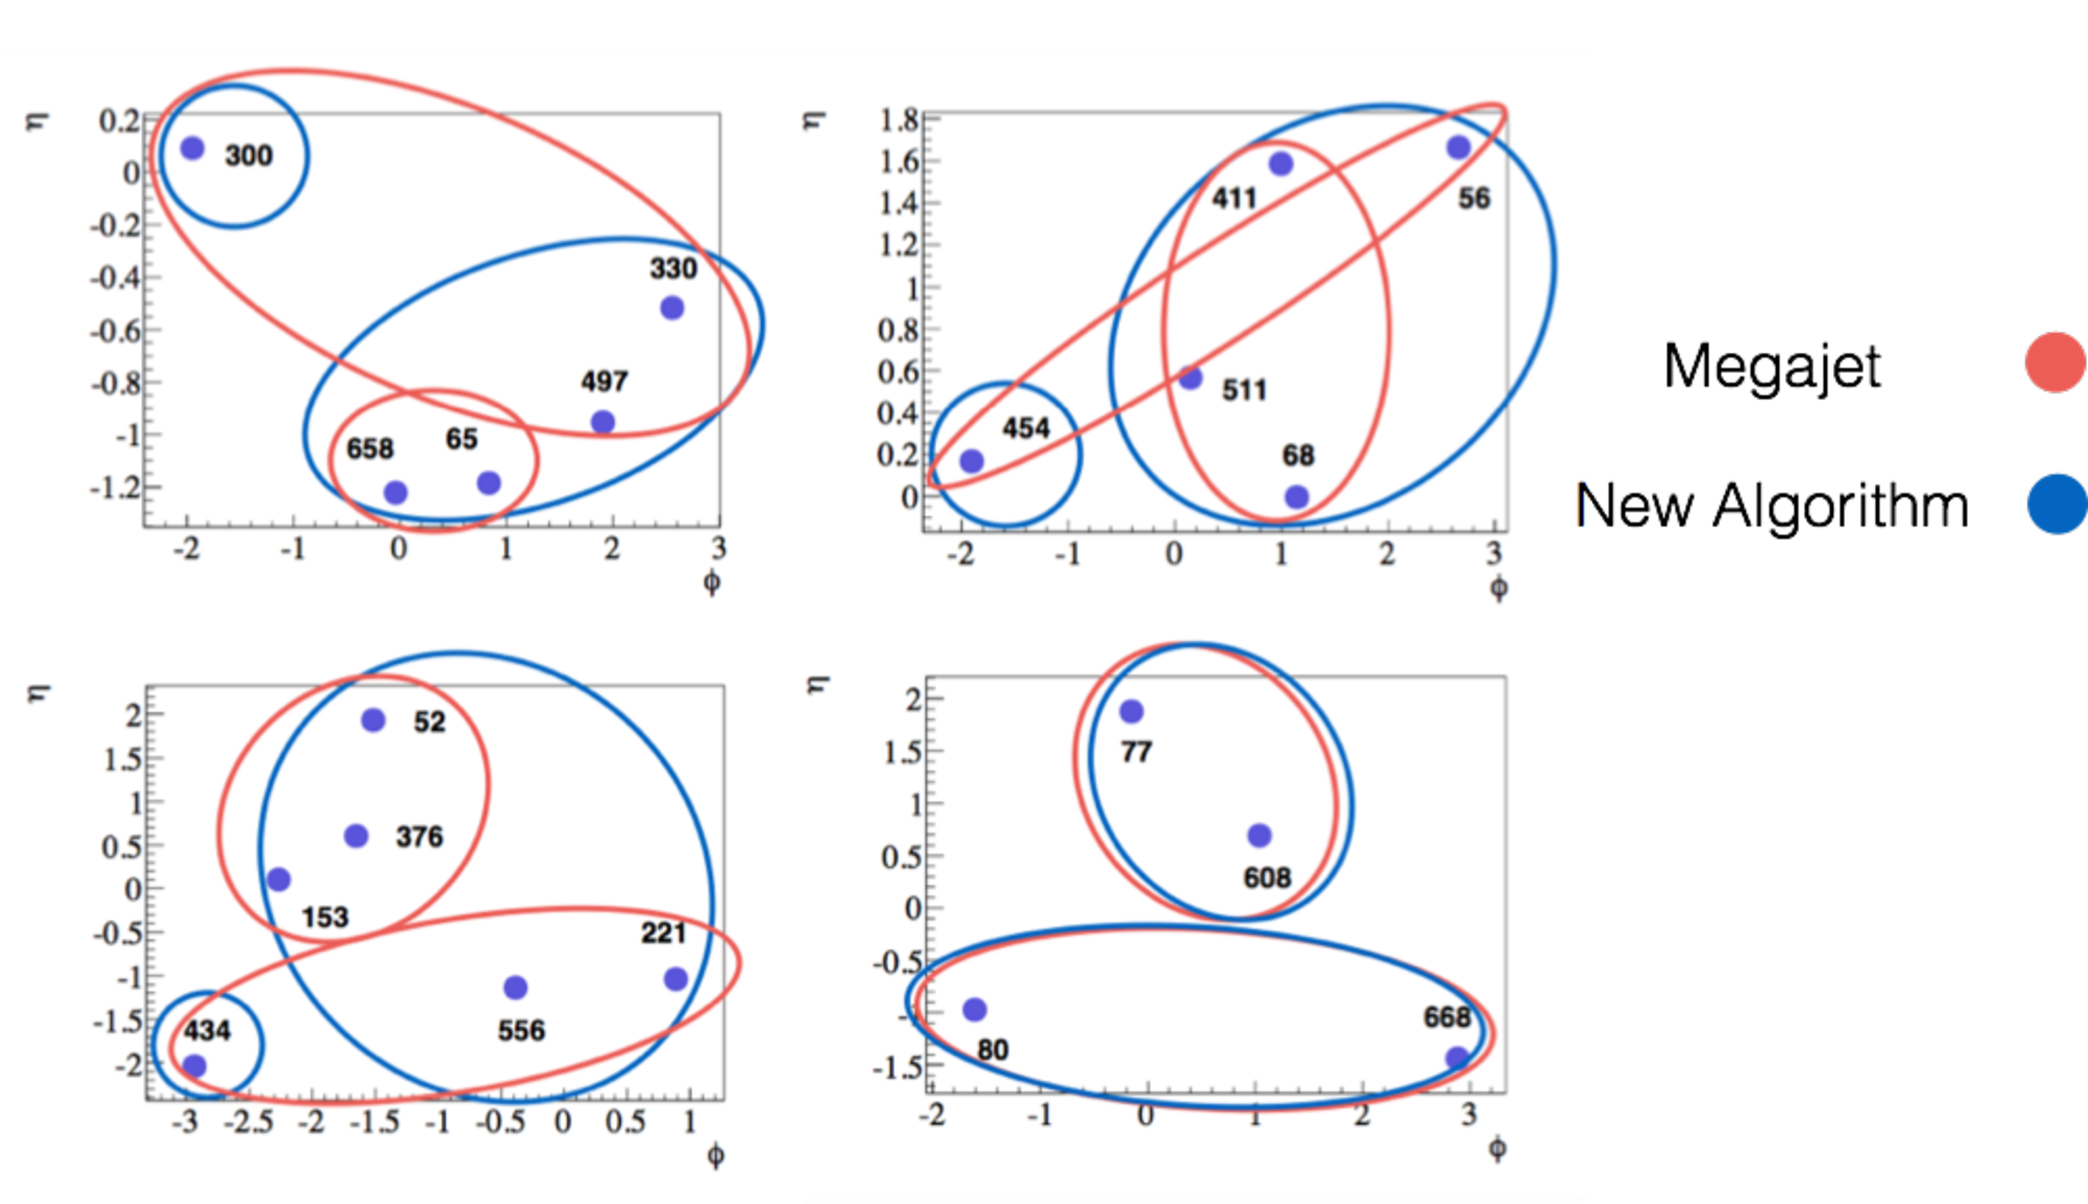
\includegraphics[width=0.98\textwidth]{eta_phi.pdf}
\caption{\label{fig:eta_phi} Clustering decisions for four independent T1 events, using the megajet and new clustering algorithms. The purple points represent the $\eta$, $\phi$ positions of the anti-KT inclusively clustered jets with R = 0.4 from the initial clustering. The adjacent numbers display their respective $p_T$ values. These jets are clustered differently into hemispheres, depending on the algorithm, and the different final states are indicated by the loops. }
\end{figure}
\end{center}
\twocolumngrid
\section{Future}
Regarding the L1 studies, the razor analyses would conclusively benefit from the implementation of the $H_T>130$ GeV \& $H_T^{miss}/H_T >$ 0.3 trigger. For the HLT, further studies must be conducted before implementation of any jet algorithm. Specifically, clustering decisions should be compared to the generator-level produced quarks, in order to determine which of the algorithms is clustering jets that originated from the decay of the same pair-produced particle. Currently, we are exploring how inclusively clustering jets would benefit the signal-to-background rejection. 
%\section{Future}
%For the upcoming weeks, a choice of which jet clustering algorithm to implement must be made. Then, efficiency studies at HLT must be conducted as well.

\section{Acknowledgments}
I would like to thank Javier Duarte for guiding me through my research, and for Maria Spiropulu for being a fantastic mentor. I would also like to express thanks for Dustin Anderson, Cristian Pena, Alex Mott, and Maurizio Pierini for their invaluable comments and guidance. Additionally, I would like to thank the entire Caltech CMS Group, with special thanks to Edward Garza for being my partner through the second half of this research. Finally, thank you to the Caltech SURF Foundation, as well as the Stanley and Chenmei Hsu Foundation for supporting my SURF. 
\bibliographystyle{apsrev4-1} % Tell bibtex which bibliography style to use
\bibliography{AnnWang/progress_report} 
\end{document}